% The master copy of this demo dissertation is held on my filespace
% on the cl file serve (/homes/mr/teaching/demodissert/)

% Last updated by MR on 2 August 2001

\documentclass[12pt,twoside,notitlepage]{report}

\usepackage{a4}
\usepackage{verbatim}
\usepackage{mathtools}% http://ctan.org/pkg/mathtools
\usepackage{etoolbox}
\usepackage{tabularx}
\usepackage{amsfonts}

% \overfence definition
\let\overfence\overbrace % \overfence is similar to \overbrace
\let\downfencefill\downbracefill % match components of \overbrace
\patchcmd{\overfence}{\downbracefill}{\downfencefill}{}{}% patch \overfence...
\patchcmd{\downfencefill}{\braceru \bracelu}{}{}{}%... and \downfencefill

% \underfence definition
\let\underfence\underbrace % \underfence is similar to \underbrace
\let\upfencefill\upbracefill % match components of \underbrace
\patchcmd{\underfence}{\upbracefill}{\upfencefill}{}{}% patch \underfence...
\patchcmd{\upfencefill}{\bracerd \braceld}{}{}{}%... and \upfencefill

\newtoggle{colourtoggle}
\newtoggle{wordcount}

\togglefalse{wordcount}




\toggletrue{colourtoggle}

\usepackage{url}
\input{epsf}                            % to allow postscript inclusions
% On thor and CUS read top of file:
%     /opt/TeX/lib/texmf/tex/dvips/epsf.sty
% On CL machines read:
%     /usr/lib/tex/macros/dvips/epsf.tex



\raggedbottom                           % try to avoid widows and orphans
\sloppy
\clubpenalty1000%
\widowpenalty1000%

\addtolength{\oddsidemargin}{6mm}       % adjust margins
\addtolength{\evensidemargin}{-8mm}

\renewcommand{\baselinestretch}{1.1}    % adjust line spacing to make
                                        % more readable



%  Listings set up
\usepackage{listings, lstlangcoq, lstlangott, lstlanglwt, bold-extra}
\usepackage{cleveref}
\crefname{lstlisting}{listing}{listings}
\Crefname{lstlisting}{Listing}{Listings}
\usepackage[usenames,dvipsnames,svgnames,table]{xcolor}

\iftoggle{colourtoggle}{
\definecolor{mygreen}{rgb}{0,0.6,0}
\definecolor{myblue}{rgb}{0,0,1}
\definecolor{myemerald}{rgb}{0.0,0.66,0.42}
\definecolor{mygray}{rgb}{0.5,0.5,0.5}
\definecolor{mymauve}{rgb}{0.58,0,0.82}
\definecolor{myseagreen}{rgb}{0.95,0.999,0.95}
}{
\definecolor{mygreen}{rgb}{0.35,0.35,0.35}
\definecolor{myblue}{RGB}{5,5,5}
\definecolor{mygray}{rgb}{0.5,0.5,0.5}
\definecolor{myemerald}{RGB}{111,111,111}
\definecolor{mymauve}{rgb}{0.25,0.25,0.25}
\definecolor{myseagreen}{rgb}{0.98,0.98,0.98}
}

\lstset{ %
  backgroundcolor=\color{myseagreen},   % choose the background color; you must add \usepackage{color} or \usepackage{xcolor}
  basicstyle=\footnotesize,        % the size of the fonts that are used for the code
  breakatwhitespace=false,         % sets if automatic breaks should only happen at whitespace
  breaklines=true,                 % sets automatic line breaking
  captionpos=b,                    % sets the caption-position to bottom
  commentstyle=\color{mygreen},    % comment style
  deletekeywords={...},            % if you want to delete keywords from the given language
  escapeinside={\%*}{*)},          % if you want to add LaTeX within your code
  extendedchars=true,              % lets you use non-ASCII characters; for 8-bits encodings only, does not work with UTF-8
  frame=shadowbox,                    % adds a frame around the code
  frameround=tttt,
  keepspaces=true,                 % keeps spaces in text, useful for keeping indentation of code (possibly needs columns=flexible)
  keywordstyle=\color{myblue},       % keyword style
  language=[Objective]Caml,        % the language of the code
  morekeywords={*,...},            % if you want to add more keywords to the set
  numbers=left,                    % where to put the line-numbers; possible values are (none, left, right)
  numbersep=5pt,                   % how far the line-numbers are from the code
  numberstyle=\tiny\color{myemerald}, % the style that is used for the line-numbers
  rulecolor=\color{myemerald},         % if not set, the frame-color may be changed on line-breaks within not-black text (e.g. comments (green here))
  showspaces=false,                % show spaces everywhere adding particular underscores; it overrides 'showstringspaces'
  showstringspaces=false,          % underline spaces within strings only
  showtabs=false,                  % show tabs within strings adding particular underscores
  stepnumber=1,                    % the step between two line-numbers. If it's 1, each line will be numbered
  stringstyle=\color{mymauve},     % string literal style
  tabsize=2,                       % sets default tabsize to 2 spaces
  title=\lstname                   % show the filename of files included with \lstinputlisting; also try caption instead of title
}

% Tikz set up
\usepackage{tikz}
\usepackage{tikz-cd}
\usetikzlibrary{arrows, shapes}

%\usepackage{harvard}

\usepackage[final]{pdfpages}

\usepackage{mathpartir}

\usepackage{float}
%\usepackage{comment}
%\excludecomment{wc}
%\includecomment{nwc}
%\renewenvironment{comment}{}{}
%\renewenvironment{lstlisting}{\begin{lstlisting}}{\end{}
%\renewenvironment{figure}{}{}
%\renewenvironment{equation}{}{}
%\renewcommand{\cite}{}

\begin{document}

\bibliographystyle{plain}


%%%%%%%%%%%%%%%%%%%%%%%%%%%%%%%%%%%%%%%%%%%%%%%%%%%%%%%%%%%%%%%%%%%%%%%%
% Title


\pagestyle{empty}

\hfill{\LARGE \bf Tam\'as Kisp\'eter}

\vspace*{60mm}
\begin{center}
\Huge
{\bf Monadic Concurrency in OCaml} \\
\vspace*{5mm}
Part II in Computer Science \\
\vspace*{5mm}
Churchill College \\
\vspace*{5mm}
\today  % today's date
\end{center}

\cleardoublepage

%%%%%%%%%%%%%%%%%%%%%%%%%%%%%%%%%%%%%%%%%%%%%%%%%%%%%%%%%%%%%%%%%%%%%%%%%%%%%%
% Proforma, table of contents and list of figures

\setcounter{page}{1}
\pagenumbering{roman}
\pagestyle{plain}

\chapter*{Proforma}

{\large
\begin{tabular}{ll}
Name:               & \bf Tam\'as Kisp\'eter                     \\
College:            & \bf Churchill College                     \\
Project Title:      & \bf Monadic Concurrency in OCaml \\
Examination:        & \bf Part II in Computer Science, July 2014        \\
Word Count:         & \bf 1587\footnotemark[1]
(well less than the 12000 limit) \\
Project Originator: & Tam\'as Kisp\'eter                    \\
Supervisor:         & Jeremy Yallop                    \\ 
\end{tabular}
}
\footnotetext[1]{This word count was computed
by {\tt detex diss.tex | tr -cd '0-9A-Za-z $\tt\backslash$n' | wc -w}
}
\stepcounter{footnote}


\section*{Original Aims of the Project}

To write an OCaml framework for lightweight threading. This framework should be defined from basic semantics and have these semantics represented in a theorem prover setting for verification. The verification should include proofs of basic monadic laws. This theorem prover representation should be extracted to OCaml where the extracted code should be as faithful to the representation as possible. The extracted code should be able to run OCaml code concurrently.



\section*{Work Completed}

All that has been completed appears in this dissertation.

\section*{Special Difficulties}

Learning how to incorporate encapulated postscript into a \LaTeX\
document on both CUS and Thor.
 
\newpage
\section*{Declaration}

I, Tam\'as Kisp\'eter of Churchill College, being a candidate for Part II of the Computer
Science Tripos, hereby declare
that this dissertation and the work described in it are my own work,
unaided except as may be specified below, and that the dissertation
does not contain material that has already been used to any substantial
extent for a comparable purpose.

\bigskip
\leftline{Signed [signature]}

\medskip
\leftline{Date \today}

\cleardoublepage

\tableofcontents

\listoffigures

\lstlistoflistings


\newpage
\section*{Acknowledgements}

%%%%%%%%%%%%%%%%%%%%%%%%%%%%%%%%%%%%%%%%%%%%%%%%%%%%%%%%%%%%%%%%%%%%%%%
% now for the chapters

\cleardoublepage        % just to make sure before the page numbering
                        % is changed

\setcounter{page}{1}
\pagenumbering{arabic}
\pagestyle{headings}
% Proforma + Intro + prep = 3100
% Implementation = 4700
% Evaluation + conclustion = 2200
% Appendicies = \infty
\chapter{Introduction}

This dissertation describes a project to build a concurrency framework for OCaml. This framework is designed with correctness in mind: developing the well defined semantics, modelled in a proof assistant and finally extracted to actual code. The project aims to be a verifiable reference implementation. 

\section{Motivation}
Verification of core libraries is becoming increasingly important as we discover more and more subtle bugs that even extensive unit testing could not find. As Dijkstra said, testing shows the presence, not the absence of bugs. On the other hand verification can show the absence of bugs, at least with respect to the formal model of the system.

Motivation of the project is to investigate the lack of certified implementation of a concurrency framework. Verified concurrent systems have been researched for languages like C\cite{sevvcik2011relaxed}, C++ and Java\cite{lochbihler2012machine}, but not yet for OCaml. 

\section{Overview of concurrency}
Concurrency is the concept of more than one thread of execution making progress in the same time period. A particular form of concurrency is parallelism, when threads physically run simultaneously.

Concurrent computation has became common in many applications in computer science with the rise of faster systems often with multiple cores. Concurrency in a computation can be exploited on several levels ranging from hardware supported instruction and thread level parallelism to software based heavy and lightweight models. 

This project aims to model lightweight, cooperative concurrency. No threads are exposed to the underlying operating system or hardware. Lightweight concurrency often provides faster switch between threads  but some blocking operations on the process level will block all internal threads. The threads in this approach expose the points of possible interleaving and the scheduling is done in software.

Most general-purpose languages offer some way of exploiting concurrency in computations. Functional programming is a good fit for concurrency, since it discourages the use of mutable data structures that lead to race conditions.  However, support for concurrency in functional languages is often lacking. Functional languages that have both actual industrial applications and large sets of features are of particular interest. These languages include OCaml and Haskell. I focused on OCaml. 
 

\section{Current implementations of a concurrency framework in OCaml}
There are two very successful monadic concurrency frameworks for OCaml. LWT\cite{LWT} and Async\cite{Async}. They both provide the primitives and syntax extensions for concurrent development. Neither is supported by a clear semantic description, because their main focus is ease of use and speed . 

LWT, the lightweight cooperative threading library\cite{vouillon2008lwt} was designed as an open source framework entirely written in OCaml in a monadic style. It was successfully used in several large projects including the Unison file synchroniser and the Ocsigen Web server. LWT includes many primitives to provide a feature rich framework, including primitives for thread creation, composition and cancellation, thread local storage and support for various synchronisation techniques. 


\begin{minipage}{\linewidth}
\begin{lstlisting}[alsolanguage={Lwt}, caption={LWT example}, label={lst:lwtsyntax}, escapeinside={@}{@}]
 open Lwt
 
 let main () =
   @\label{lst:lwtsyntaxHeadsDefStart}@let heads =
     Lwt_unix.sleep 1.0 >>
     @\label{lst:lwtsyntaxHeadsDefEnd}@return (print_endline "Heads");
   in
@\label{lst:lwtsyntaxTailsDefStart}@   let tails =
     Lwt_unix.sleep 2.0 >>
@\label{lst:lwtsyntaxTailsDefEnd}@     return (print_endline "Tails");
   in
@\label{lst:lwtsyntaxThreadStart}@   lwt () = heads <&> tails in
@\label{lst:lwtsyntaxThreadEnd}@   return (print_endline "Finished")
 
 let _ = Lwt_main.run (main ())
\end{lstlisting}
\end{minipage}



In \Cref{lst:lwtsyntax} we can see some of the syntax of LWT. Lines \ref{lst:lwtsyntaxHeadsDefStart}--\ref{lst:lwtsyntaxHeadsDefEnd} define heads, a function that sleeps for 1 second and then prints "Head", and lines \ref{lst:lwtsyntaxTailsDefStart}--\ref{lst:lwtsyntaxTailsDefEnd} define tails which sleeps for 2 seconds and then prints "Tails".  Lines \ref{lst:lwtsyntaxThreadStart}--\ref{lst:lwtsyntaxThreadEnd} create a thread that waits on heads and tails and then prints "Finished".  In LWT, semantics mostly follow the principle of continuations. We build a sequence of computations and the scheduler can pick between parallel computations at points of sequencing.

An other implementation, Async is an open source concurrency library for OCaml developed by Jane Street. Unlike LWT the basic semantics are designed with promises in mind. A promise is a container that can be used in place of a value of the same type, but computations with a promise only evaluate when the actual value has been calculated. The concurrency arises naturally by interleaving the fulfilment of these containers. 


\begin{minipage}{\linewidth}
\begin{lstlisting}[caption={Async example}, label={lst:asyncsyntax},escapeinside={@}{@}]
open Core.Std
open Async.Std

let heads=(after (sec 1.0)  >>| fun () -> (print_endline "Heads"))
let tails=(after (sec 2.0)  >>| fun () -> (print_endline "Tails"))
let head_and_tails = (Deferred.both
   heads
   tails)


let () = upon (head_and_tails) (fun _ -> ())
  
let () = never_returns (Scheduler.go ())
\end{lstlisting}
\end{minipage}



In \Cref{lst:asyncsyntax} we define \verb|heads| and \verb|tails| as Deferred values of the respective code sequences. A Deferred is an implementation of a promise.


There are a number of other experimental implementations of concurrency in OCaml. For example JoCaml\cite{jocaml} implements join calculus over OCaml, Functory\cite{functory} focuses on distributed computation, OCamlNet exploits multiple cores and OCamlMPI\cite{ocamlmpi} provides bindings for the standard MPI message passing framework.


\section{Semantics of concurrency}

There has been a lot of work on formulating the semantics of concurrent and distributed systems. Some of the most common models for lightweight concurrency\cite{deleuzelight} are captured\cite{friedman1988applications} and delimited\cite{kiselyov2010delimited} continuations\cite{shan2004shift}, trampolined style\cite{ganz1999trampolined}, continuation monads\cite{Claessen99functionalpearls}, promise monads\cite{liskov1988promises} and event based programming (as used, for example in the OCamlNet\cite{Ocamlnet} project). This work focuses on the continuation monad style.

A monad\cite{hoareetal2001tackling} in functional programming is a construct to structure computations that are in some sense "sequenced" together. This sequencing can be for example string concatenation, simple operation sequencing (the well known semicolon of imperative programming) or conditional execution. Two operations commonly called bind and return and a type constructor of a parametric type, like $ \alpha \, M $ where $ \alpha $ is any type, form a monad when they obey a set of axioms called monadic laws.

Most monads support further operations and a concurrency monad is one such monad. Beside the two necessary operations (return and bind) a concurrency monad has to support at least one that deals with concurrent execution.  This operation can come in many forms and under many names, for example fork, join or choose. Each with differing signatures and semantics:
\begin{itemize}
\item{Fork would commonly take two different computations and evaluate them together. Its return semantics would be to return when one thread finished but include the partially completed other computation if possible.}
\item{Join may take many threads, but it waits for all threads to finish.}
\item{Choose can also take many computations, however it would commonly either only evaluate one thread or discard every thread but the one that finished first.}
\end{itemize}

\section{Semantics to logic}
The semantics of concurrency can be modelled in logic, in particular logics used by proof assistants. The developer can use this model to formally verify properties about the semantics\cite{benton2008mechanized,blazy2009mechanized,blazy2006formal,leroy2009formal}. Coq\cite{Coq}, HOL and Isabelle are widely used proof assistants. Tools like Ott\cite{Ott} help with the modelling process with ascii-art notation and translation to proof assistants and \LaTeX.


\section{Logic to runnable code}
While a number of proof assistants have utilities for direct computation, in most cases semantics is described as a set of logical, not necessarily constructive relations. This representation is more amenable to proofs than to actual execution, because there is no need for an input-output relationship. Without this strict requirement on the relation the representation can be more succinct, but hard to extract. Letouzey\cite{letouzey2008extraction} has shown that many such definitions can be extracted into executable OCaml or Haskell code.  Coq and Isabelle provide tools for this extraction. The tools also generate a proof that the extracted code is faithful to the representation in the proof assistant.


\chapter{Preparation}
During the preparation phase of this project many decisions had to be made, including the concurrency model, large scale semantics and the tool chain used in the process.

\section{Design of concurrent semantics}
%Brief overview of techiniques for concurrency
Concurrency may be modelled in many ways. A popular way of modelling concurrency is with a process calculus. A process calculus is an algebra of processes or threads where. A thread is a unit of control, sometimes also a unit of resources. This algebra often comes with a number of operations like 
\begin{itemize}
\item{$ P\, | \, Q $  for parallel composition where $ P $ and $ Q $ are processes}
\item{ $ a.P  $ for sequential composition where $ a $ is an atomic action and $ P $ is a process executed sequentially}
\item{$ !P $ for replication where $ P $ is a process and $ !P \equiv P \, | \, !P $}
\item{$ x\langle y \rangle \cdot P $ and $ x(v) \cdot Q $ for sending and receiving messages through channel $ x $ respectively} 
\end{itemize}

%Process calculus ?

%Choices for concurrency semantics
This project aimed to have simple but powerful operational semantics. Simplicity is required in both the design and the interface. There is a short and limited timespan for implementation and an even shorter period for the user to understand the system. On the other hand, the model should have comparable formal properties to full, well known process calculi. 

I focused on providing primitives for operations on processes including parallel and sequential composition and recursion. Formal treatment of communication channels have been left out to limit the scope of the project.  


\section{Choice of implementation style}  
%Why I chose continuation monads vs. World
Deleuze\cite{deleuzelight} surveyed a number of implementation styles of lightweight concurrency for OCaml. The styles fall in two broad categories: direct and indirect styles. Direct styles like captured and delimited continuations involve keeping an explicit queue of continuations that can be executed at any given time and a scheduler that picks the next element from the queue. Indirect styles include the trampolined style and two monadic styles: continuations and promises.

Simplicity and similarity to current implementations like LWT and Async were the two factors in the decision between these styles. Both direct styles and the promise monad style keep concurrency state data that is external to the language and has to be maintained at runtime explicitly. The extra structure would make the implementation slightly more complex. LWT and Async both provide monadic style interfaces therefore I chose the continuation monad style.





\section{Design of monadic semantics}
Category theory has been a general tool used to model functional programming languages and programs. Monads are a concept originating from this connection. 


A monad on a category $ C $ is a triple $ (T, \eta, \mu) $ where $ T $ is an endofunctor on $ C $, that is, it maps the category to itself. The last two, $ \eta $ and $ \mu $ are natural transformations such that $ \eta:\, 1_C \rightarrow T $, that is between the identity functor and $ T $, and $ \mu:\, T^2 \rightarrow T $. The first transformation, $ \eta $ describes a lift operation: essentially we can wrap the object in $ C $ and preserving its properties. The second transformation, $ \mu $ is about an operation called join. This operation unwraps a layer of wrapping if there are two. To call a triple like this a monad it has to satisfy two conditions, called coherence conditions.
\begin{enumerate}

\item{
\iftoggle{wordcount}{}{
\[ \mu \circ T \mu = \mu \circ \mu T \]
}
Or as commutative diagram:
\begin{center}
\begin{tikzcd}
T^3 \arrow{r}{T\mu} \arrow{d}[swap]{\mu T}
& T^2 \arrow{d}{\mu} \\
T^2 \ar{r}[swap]{\mu} & T
\end{tikzcd}
\end{center}
This property roughly demands that unwrapping from three layers to one is associative.



}
\item{
\[ \mu \circ T\eta = \mu \circ \eta T = 1_T \]

Or as commutative diagram:
\begin{center}
\begin{tikzcd}
T \arrow{r}{\eta T} \arrow{d}[swap]{T \eta } \arrow[equal]{rd}
& T^2 \arrow{d}{\mu} \\
T^2 \ar{r}[swap]{\mu} & T
\end{tikzcd}
\end{center}

That is to say wrapping and then subsequently unwrapping behaves as an identity.
}
\end{enumerate}

This description entails three operations (lift, join and map) and their behaviour (associativity and identity), however this is a formulation rarely used in practice. There is an equivalent pair of operations (ret and bind) with similar behaviour constraints that is used in most monadic programming constructs. 


Most implementations go along the following lines: there is a parametric type $ \textbf{con} \, \alpha $ where $ \alpha $ is the type parameter. Note $ \textbf{con} $ is an arbitrary name, marker for a particular monad. The I/O monad would have IO as the marker.

The \lstinline|ret| takes a value of the language and gives its monadic counterpart. With types \lstinline|ret| can be represented as $ \textbf{ret} \, :\, \forall \alpha. \alpha\, \rightarrow\, \textbf{con}\, \alpha $.

The \lstinline|bind| (often written as $ \gg= $)  takes a monadic value (that is one in the parametric type $ \textbf{con} \, \alpha $) and a function that can map the inner value to a new monadic value (that is, it has type $ \alpha \, \rightarrow \, \textbf{con} \, \beta $). Bind then returns a $ \textbf{con} \, \beta $. With types $ \gg= $ means: $ \gg= \, : \, \forall \alpha \, \beta. \; \textbf{con} \, \alpha \rightarrow (\alpha \rightarrow \textbf{con} \, \beta) \rightarrow \textbf{con} \, \beta $.

To call this system a monad, we need to satisfy three axioms:

\begin{enumerate}
\item{\lstinline|ret| is essentially a left neutral element:
\[ (\textbf{ret} \, x) \, \gg=\, f \quad \equiv \quad f \, x \]}
\item{\lstinline|ret| is essentially a right neutral element:
\[ m \, \gg=\, \textbf{ret} \quad \equiv \quad m \]}
\item{\lstinline|bind| is associative:
\[ (m \, \gg= \, f) \, \gg= g \quad \equiv \quad m\, \gg= \, (\lambda\, x. (f\, x \, \gg= \, g) ) \]}
\end{enumerate}

We will return to the exact nature of $ \equiv $ used in this project in the evaluation section.


\section{Tools}
The project uses a chain of three tools: \begin{enumerate}
\item{
Ott, a tool for transforming informal, readable semantics to both \LaTeX and formal proof assistant code.}
\item{Coq, a proof assistant supported by Ott. }
\item{OCaml, the target language. }
\end{enumerate}

\begin{figure}[h!]
\centering

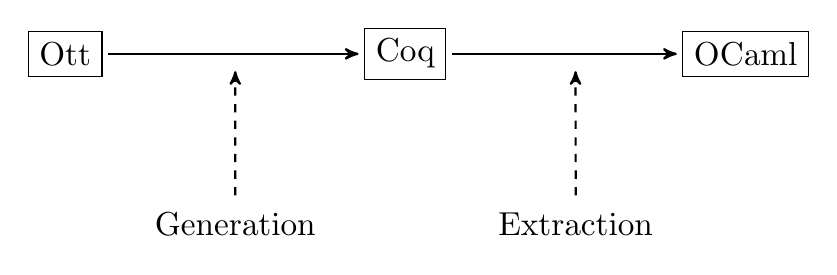
\begin{tikzpicture}[node distance=1.8cm, auto, >=stealth',pil/.style={
           ->,
           thick,
           shorten <=2pt,
           shorten >=2pt,}, pildashed/.style={
                      ->,
                      thick,
                      dashed,
                      shorten <=2pt,
                      shorten >=2pt,},scale=1.2, every node/.style={scale=1.2}, ]
\node[draw, rectangle] (o) {Ott};
\node[right of=o] (otch) {};
\node[below of={otch}] (otc) {Generation}
  edge[pildashed] (otch);
\node[draw, rectangle, right of={otch}] (c) {Coq}
  edge[pil, <-] (o);
\node[right of=c] (ceoh) {};
\node[below of={ceoh}] (ceo) {Extraction}
  edge[pildashed] (ceoh);
\node[draw, rectangle, right of={ceoh}] (oc) {OCaml}
  edge[pil, <-] (c);

\end{tikzpicture}
\caption{High level view of the tool chain}
\end{figure}

In the preparation phase I got acquainted with all three of these systems, as I have not used them before for any serious work.
\subsection{Ott}
% Why Ott (because it is awesome)
To avoid duplication of the semantics in several formats I have to chosen to use a supporting tool called Ott. It enables the use of a simple ASCII-art like description of grammars, typing and reduction relations. Ott can export to various destination formats including most proof assistants and \LaTeX. The Ott  is the primary form of the semantics that all further forms are derived from in the project.

For someone familiar to formal semantics Ott has an easy to use and intuitive syntax. 

Metavariables used in productions are defined with their destination language equivalents and potentially (in the case of Coq) their equality operation.
\begin{lstlisting}[language={Ott}, caption={Ott metavariable definition}]
metavar termvar, x ::=   {{ com  term variable }} 
{{ isa string}} {{ coq nat}} {{ hol string}} {{ coq-equality }}
{{ ocaml int}} {{ lex alphanum}} {{ tex \mathit{[[termvar]]} }}
\end{lstlisting}

Term expression grammars and other grammars can be defined in the well known Backus-Naur form with some extensions.

\begin{lstlisting}[language={Ott}, caption={Ott grammar example}, label={lst:ottgrammarex}]
grammar
t :: 't_' ::=                                 {{ com term    }}
  | x            ::  :: Var                   {{ com variable}}
  | \ x . t      ::  :: Lam (+ bind x in t +) {{ com lambda  }}
  | t t'         ::  :: App                   {{ com app     }}
  | ( t )        :: S:: Paren                 {{ icho [[t]]  }} 
  | { t / x } t' :: M:: Tsub  
                        {{ icho (tsubst_t [[t]] [[x]] [[t']])}}
\end{lstlisting}

In \Cref{lst:ottgrammarex} the non-terminal t for terms is defined with 5 productions: variables, lambda abstractions, applications, parentheses grouping and variable substitution. Each of these rules have a name, for example Var and Lam. Each of these names are prefixed by the unique prefix t\_ to have non-ambiguous names. The right hand side of each line describes the translation to target languages, for example com will  generate the given description for the \LaTeX\, target. 

There are meta flags S and M to describe syntactical sugar and meta productions that are not generated as data structure elements in target languages, but instead have their own instructions: for example the substitution term will be rewritten as an application of the tsubst\_t relation defined elsewhere. 

In many languages one might want to define a value subgrammar, which can be used both in the reduction relation definition and in proving properties of the semantics. Ott has support for general subgrammar relation check.
\begin{lstlisting}[language={Ott}, caption={Ott value subgrammar example}, label={lst:ottvaluesubgrammarexample}]
v :: 'v_' ::=                                 {{ com value   }}
  | \ x . t      ::  :: Lam                   {{ com lambda  }}
  
subrules
  v <:: t
\end{lstlisting}
In \Cref{lst:ottvaluesubgrammarexample} v is a subgrammar of t. The statement v $<::$ t is exported as a target language subroutine that checks whether the value relation holds and during translation Ott checks for obvious bugs.

Another common feature of semantics is substitution of values for variables, for example in function application. Substitution is so frequent that Ott provides both single and multiple variable substitutions for the target languages as subroutines in the translated code.




\begin{minipage}{\linewidth}
\begin{lstlisting}[language={Ott}, caption={Ott substitution example}, label={lst:ottsubstex}]
substitutions
  single t x :: tsubst 
\end{lstlisting}
\end{minipage}


The statement \lstinline[language={Ott}]|single t x :: tsubsts| in \Cref{lst:ottsubstex} defines a single substitution function called tsubsts\_t over terms defined by the grammar for t and for variables represented by the metavariable x. This is the relation mentioned in the grammar for the target language version for \{ t / x \} t'.



Finally paramount to most semantics are relations like the reduction relation.
\begin{lstlisting}[language={Ott}, caption={Ott reduction relation example}, label={lst:ottredex}]
defns
Jop :: '' ::=

 defn
 t1 --> t2 :: ::reduce::'' {{ com [[t1]] reduces to [[t2]]}} by


    --------------------------  :: ax_app
    (\x.t12) v2 -->  {v2/x}t12

    t1 --> t1'
    -------------- :: ctx_app_fun
    t1 t --> t1' t

    t1 --> t1'
    -------------- :: ctx_app_arg
    v t1 --> v t1'
\end{lstlisting}
In \Cref{lst:ottredex} I define a set of mutually recursive relations named Jop with one relation in it the $-->$ or reduce relation. Each element of this relation takes the form t1 $-->$ t2, where t1 and t2 are both terms of the grammar defined above. There are three statements for function application: the actual substitution, reduction of the first term and reduction of the second term. 
\begin{lstlisting}[language={Ott}, caption={Ott single reduction}]
t1 --> t1'
-------------- :: ctx_app_fun
t1 t --> t1' t
\end{lstlisting}
The premise(s) appear line-by-line above the ascii-art line, while and the result below the line. Next to the line is the name of the statement which is then prefixed by the name of the relation to avoid ambiguity. 



\subsection{Coq}
% Brief overview of proof assistants, reason for the choice of Coq
There are a number of proof assistants available as destinations for Ott, out of which Coq and Isabelle provide good extraction facilities to OCaml. They are at a glance rather similar. The choice between the two came down to advice from supervisors as I did not have experience with either systems. This project was developed with the Coq proof assistant. 

Coq is formal proof assistant with a mathematical higher-level language called \textit{Gallina}, based around the Calculus of Inductive Constructions, that can be used to define functions and predicates, state, formally prove and machine check mathematical theorems and extract certified programs to high level languages like Haskell and OCaml.
% Short guide to reading Coq

Objects in Coq can divided into two sorts, \textit{Prop} (propositions) and \textit{Type}. A proposition like $ \forall A, B.\; A \wedge B \rightarrow B \vee B $ translates to the snippet in \Cref{lst:coqproplogex}.

\begin{lstlisting}[language={Coq},caption={Coq Prop logic example},label={lst:coqproplogex}]
forall A B : Prop, A /\ B -> B \/ B
\end{lstlisting}

Predicates like equality and other sets can be used as well.

\begin{lstlisting}[language={Coq},caption={Coq Prop predicate example}]
forall x y : Z, x * y = 0 -> x = 0 \/ y = 0
\end{lstlisting}

New predicates can be defined inductively

\begin{lstlisting}[language={Coq},caption={Coq Prop new predicate example}]
 Inductive even : N -> Prop :=
  | even_0 : even 0
  | even_S n : odd n -> even (n + 1)
  with odd : N -> Prop :=
  | odd_S n : even n -> odd (n + 1).
\end{lstlisting}

Data structures can also be defined both inductively and coinductively.

\begin{lstlisting}[language={Coq},caption={Coq inductive data structure example}]
 Inductive seq : nat -> Set :=
  | niln  : seq 0
  | consn : forall n : nat, nat -> seq n -> seq (S n).
\end{lstlisting}

\begin{lstlisting}[language={Coq},caption={Coq coinductive data structure example}]
 CoInductive stream (A:Type) : Type :=
  | Cons : A -> stream -> stream.
\end{lstlisting}

Functions over these data structures are defined as fixpoints and cofixpoints respectively.

\begin{lstlisting}[language={Coq},caption={Coq fixpoint example}]
 Fixpoint length (n : nat) (s : seq n) {struct s} : nat := 
     match s with
     | niln => 0
     | consn i _ s' => S (length i s')
     end.
\end{lstlisting}

Finally theorems can be proven with these propositions and structures.

\begin{minipage}{\linewidth}
\begin{lstlisting}[language={Coq},caption={Coq theorem example}]
Theorem length_corr : forall (n : nat) (s : seq n), length n s = n.
  Proof.
    intros n s.

    (* reasoning by induction over s. Then, we have two new goals
       corresponding on the case analysis about s (either it is 
       niln or some consn *)
    induction s.

      (* We are in the case where s is void. We can reduce the 
         term: length 0 niln *)
      simpl. 

      (* We obtain the goal 0 = 0. *)
      trivial.

      (* now, we treat the case s = consn n e s with induction 
         hypothesis IHs *)
      simpl. 

      (* The induction hypothesis has type length n s = n. 
         So we can use it to perform some rewriting in the goal: *)
      rewrite IHs. 

      (* Now the goal is the trivial equality: S n = S n *)
      trivial.

    (* Now all sub cases are closed, we perform the ultimate
       step: typing the term built using tactics and save it as
       a witness of the theorem. *)
  Qed.	  
\end{lstlisting}
\end{minipage}
Each Lemma, Theorem, Example have a name and a statement. The statement is a proposition. This is followed by the proof in which a sequence of steps modify the assumed hypotheses and the goal proposition until it has been proven. These steps are called tactics which can be simple application of previous theorems and axioms or as complex as a SAT solver. Coq comes with a language Ltac to allow users to build their own tactics.

% Methods of extraction

Coq also provides built in facilities for the certified extraction of code to OCaml, Haskell and Scheme. These can be invoked with the keywords \lstinline[language={Coq}]|Extraction| and \lstinline[language={Coq}]|Recursive Extraction|. 


\begin{minipage}{\linewidth}
\begin{lstlisting}[caption={Coq to OCaml extraction of seq}]
type nat =
| O
| S of nat

type seq =
| Niln
| Consn of nat * nat * seq
\end{lstlisting}
\end{minipage}

\begin{minipage}{\linewidth}
\begin{lstlisting}[caption={Coq to OCaml extraction of length}]
(** val length : nat -> seq -> nat **)

let rec length n = function
| Niln -> O
| Consn (i, n0, s') -> S (length i s')
\end{lstlisting}
\end{minipage}

% Extraction plugin

Out of the box, Coq does not provide facilities for the extraction of so called logical inductive systems. These are essentially inductively defined propositions.


\begin{minipage}{\linewidth}
\begin{lstlisting}[language={Coq},caption={Coq logical inductive example}]
Inductive add : nat -> nat -> nat -> Prop :=
| addO : forall n , add n O n
| addS : forall n m p, add n m p -> add n (S m) (S p).
\end{lstlisting}
\end{minipage}

However with the help of a plugin developed by David Delahaye, Catherine Dubois, Jean-Fr\'ed\'eric \'Etienne and Pierre-Nicolas Tollitte \cite{delahaye2007extracting,tollitte2012producing} by marking different modalities of the inductively generated proposition we can generate code with an input-output convention.



\begin{minipage}{\linewidth}
\begin{lstlisting}[language={Coq},caption={Coq to OCaml extraction of a logical inductive relation}]
(** val add12 : nat -> nat -> nat **)

let rec add12 p1 p2 =
  match (p1, p2) with
  | (n, O) -> n
  | (n, S m) ->
    (match add12 n m with
     | p -> S p
     | _ -> assert false (*  *))
  | _ -> assert false (*  *)
\end{lstlisting}
\end{minipage}

Most descriptions of reduction relations and indeed the output of Ott is of this kind, therefore this plugin helps with the extraction of a reduction relation directly. 

\subsection{OCaml}
% Brief overview of OCaml
OCaml is a high level programming language. It combines functional, object-oriented and imperative paradigms and used in large scale industrial and academic projects where speed and correctness are of utmost importance. OCaml uses one of the most powerful type and inference systems available to make efficient and correct software engineering possible.

OCaml, like many other functional languages support a wide range of features, from simple functions, to mutually recursive functions with pattern matching.
\begin{minipage}{\linewidth}
\begin{lstlisting}[caption={OCaml simple function example: square}]
let square x = x * x
\end{lstlisting}
\end{minipage}



\begin{minipage}{\linewidth}
\begin{lstlisting}[caption={OCaml recursive function example: factorial}]
let rec fact x =
    if x <= 1 then 1 else x * fact (x - 1)
\end{lstlisting}
\end{minipage}

\begin{minipage}{\linewidth}
\begin{lstlisting}[caption={OCaml complex function example: insertion sort}]
let rec sort = function
    | [] -> []
    | x :: l -> insert x (sort l)
  and insert elem = function
    | [] -> [elem]
    | x :: l -> if elem < x then elem :: x :: l
                else x :: insert elem l
\end{lstlisting}
\end{minipage}

Furthermore, it was designed as a versatile, general purpose programming language. OCaml features include objects, modules, support for imperative style and higher order functions.

\begin{minipage}{\linewidth}
\begin{lstlisting}[caption={OCaml imperative function example}]
let add_polynom p1 p2 =
    let n1 = Array.length p1
    and n2 = Array.length p2 in
    let result = Array.create (max n1 n2) 0 in
    for i = 0 to n1 - 1 do result.(i) <- p1.(i) done;
    for i = 0 to n2 - 1 do result.(i) <- result.(i) + p2.(i) done;
\end{lstlisting}
\end{minipage}

\begin{minipage}{\linewidth}
\begin{lstlisting}[caption={OCaml higher order functions example}]
let rec sigma f = function
    | [] -> 0
    | x :: l -> f x + sigma f l
\end{lstlisting}
\end{minipage}
    
\begin{minipage}{\linewidth}
\begin{lstlisting}[caption={OCaml data structure example}]
type expression =
    | Num of int
    | Var of string
    | Let of string * expression * expression
    | Binop of string * expression * expression
\end{lstlisting}
\end{minipage}
    
\begin{minipage}{\linewidth}
\begin{lstlisting}[caption={OCaml evaluation function example}]    
let rec eval env = function
    | Num i -> i
    | Var x -> List.assoc x env
    | Let (x, e1, in_e2) ->
       let val_x = eval env e1 in
       eval ((x, val_x) :: env) in_e2
    | Binop (op, e1, e2) ->
       let v1 = eval env e1 in
       let v2 = eval env e2 in
       eval_op op v1 v2
  and eval_op op v1 v2 =
    match op with
    | "+" -> v1 + v2
    | "-" -> v1 - v2
    | "*" -> v1 * v2
    | "/" -> v1 / v2
    | _ -> failwith ("Unknown operator: " ^ op)
\end{lstlisting}
\end{minipage}


% Short guide to reading OCaml

\cleardoublepage
\chapter{Implementation}
This concurrency framework was implemented as a small language of expressions and a reduction relation. These two were then translated to OCaml as constructors and an evaluation function respectively. To use the framework the user constructs an expression of the language, including within the expression the computations he wants to evaluate. The expression is than passed the evaluation function.  This language provides tools for sequencing, running computations in parallel and to make decisions based on what computations have finished. The implementation of the language was done in 6 stages as shown in \Cref{fig:detailedimploutline}. 
\begin{figure}[h]
\begin{center}
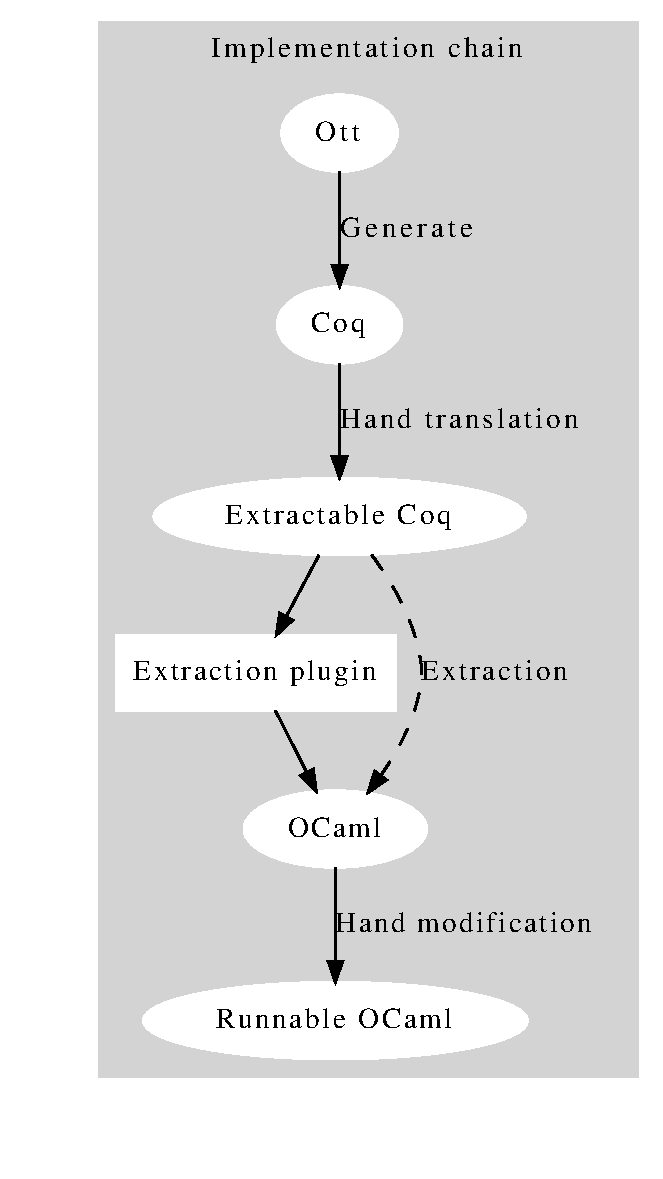
\includegraphics[scale=0.5]{implOut}
\caption{Detailed outline of the implementation}
\label{fig:detailedimploutline}
\end{center}
\end{figure}

The overall semantics were defined in Ott. These semantics were then extracted to Coq by Ott in a logical inductive format. This format, as previously mentioned, is well suited for proofs, but not for extraction. Furthermore, Ott did not correctly handle values that are partial applications of primitives taking more than one argument (\textbf{fork} and \textbf{pair}). The incorrect value predicate is fixed in the Modified Coq stage appearing in \Cref{fig:detailedimploutline}. This is the only change.

I modified the logical inductive format of the semantics in the Extractable Coq stage to have a well formed input for the extraction plugin. This plugin will be detailed later. After the extraction the generated OCaml contains computation place holders and unused labels for the transitions. I replace these place holders with the actual computations and provide some syntactic sugar, as the generated OCaml is rather cumbersome to write in.
\section{The semantics}
In this section I will describe the implemented semantics. These semantics were written in Ott. Much of the inspiration for the semantics of basic features comes from Benjamin C. Pierce: \textit{Types and Programming Languages}\cite{pierce2002types}. The Ott code was based on the simply typed $ \lambda $-calculus and polymorphic $ \lambda $-calculus examples provided with the tool\cite{Ott}. For a \LaTeX\, render of the full semantics as produced by Ott see \cref{chap:fullsemantics}.

The language of this concurrency framework is simply typed. 

The reduction semantics is given as small step labelled transitions. Small step semantics means that there is a reduction relation that is between two expressions $ e, \, e' $ where $ e $ can directly and atomically transition to $ e' $. Labelled transitions further extend this idea. In this project I used a 4-tuple $ (e, s, rl, e') $ of the starting expression, a selection operator that will be supplied by a scheduler to pick between potential reductions, a reduction label that describes the observable action and the ending expression of the transition. What this four tuple means that given the selection operator, which may be 1 or 2, given $ e $ as a starting expression can move to $ e' $ and with an effect $ rl $. This $ rl $ may be an atomic action $ l $ that can be observed or be $ \tau $ which is a silent action. Silent actions are not observed from the outside. I used the notation $ e \overset{rl}{\underset{s}{\longrightarrow}} e' $.
 
The semantics splits into three main parts
\begin{enumerate}
\item{Grammars:\begin{itemize}
\item{expressions}
\item{values}
\item{constants}
\item{types}
\item{terminals}
\end{itemize}
For the dependence between different parts of the grammars, see \Cref{fig:grammardep}.}
\item{Type judgements}
\item{Reduction judgements}
\end{enumerate}
\begin{figure}[h]
\begin{center}
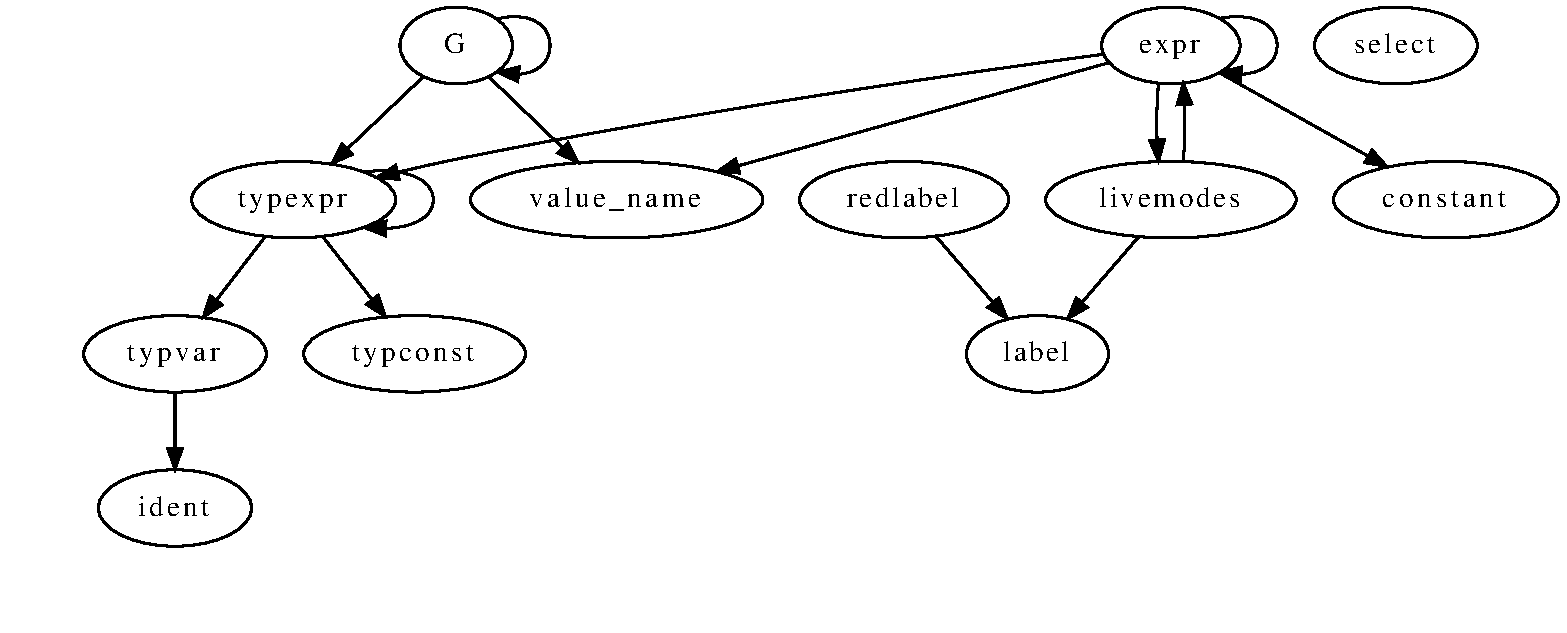
\includegraphics[width=\linewidth]{./../mconbaseDep}
\caption{Grammar dependencies}
\label{fig:grammardep}
\end{center}
\end{figure}

I will detail the semantics feature-by-feature: arrow types or functions, sum types or tagged unions, product types or pairs, the fixpoint combinator, the monadic primitives and the fork operator. The presentation of semantics for each of the features were inspired by Pierce\cite{pierce2002types}. Each section will have a corresponding table of syntax, evaluation rules and typing rules.  In the syntax section I will introduce every new syntactic form used in the evaluation and typing rules, but I will not repeat previously mentioned syntax. The presentation of both the syntax and the evaluation and typing rules were slightly simplified for better readability.  

\subsection{Arrow types}
\begin{figure}[h!]
  \centering
  $\underbracket{\overbracket{\textrm{
  \begin{tabular}{l | l}
    \begin{minipage}{0.6\linewidth}
    \begin{tabularx}{\textwidth}{l l >{\raggedleft}X}
    \textit{Syntax} &  & \tabularnewline
    e\, ::=  &  & \textit{terms:}\tabularnewline
      & x  & \textit{value name}\tabularnewline
      & $ \lambda $x:T.e  & \textit{abstraction}\tabularnewline
      & e e  & \textit{application}\tabularnewline
      &   & \tabularnewline
      v\, ::=  &  & \textit{values:}\tabularnewline
      & $ \lambda $x:T.e  & \textit{abstraction value}\tabularnewline
      &   & \tabularnewline
      T\, ::=  &  & \textit{types:}\tabularnewline
      & TV  & \textit{type variable}\tabularnewline
      & T$ \rightarrow $T  & $ \rightarrow $ \textit{type}\tabularnewline
      &   & \tabularnewline
      $ \Gamma $\, ::=  &  & \textit{contexts:}\tabularnewline
      & $ \emptyset $  & \textit{empty context}\tabularnewline
      & $ \Gamma,  $ x:T  & \textit{term variable binding}\tabularnewline 
      &   & \tabularnewline
      $ rl $\, ::=  &  & \textit{labels:}\tabularnewline
      & $ \tau $  & \textit{silent}\tabularnewline
      & $ l $  & \textit{action}\tabularnewline
      &   & \tabularnewline
      $ s $\, ::=  &  & \textit{select:}\tabularnewline
      & $ 1 $  & \textit{first}\tabularnewline
      & $ 2 $  & \textit{second}\tabularnewline      
    \end{tabularx}
    \end{minipage} & \begin{minipage}{0.40\linewidth}
        \begin{tabular}{l}
        \begin{minipage}{\textwidth}
         \begin{tabularx}{\textwidth}{>{\raggedright}X}
             \textit{Evaluation} \hfill \fbox{$e \, \overset{rl}{\underset{s}{\longrightarrow}} \, e'$}  \tabularnewline   \begin{equation}
                                     \inferrule
                                       {  }
                                       { ( \lambda\, x\,:\,T. e)\, v \overset{\tau}{\underset{s}{\longrightarrow}} \{v / x\}e } \tag{R-Subst}
                                     \end{equation} \vspace{-9mm}
                                     \tabularnewline   \begin{equation}
                                      \inferrule
                                       { e \overset{rl}{\underset{s}{\longrightarrow}} e''}
                                       { e\,e' \, \overset{rl}{\underset{s}{\longrightarrow}}\, e''\, e'\,  } \tag{R-App1}
                                       \end{equation}\vspace{-9mm}
                                     \tabularnewline   \begin{equation}
                                     \inferrule
                                      { e' \overset{rl}{\underset{s}{\longrightarrow}} e''}
                                      { v\,e' \, \overset{rl}{\underset{s}{\longrightarrow}}\, v\, e''\,  } \tag{R-App2}
                                                               \end{equation}
             \end{tabularx}
        \end{minipage} \\ 
        \begin{minipage}{\textwidth}
           \begin{tabularx}{\textwidth}{>{\raggedright}X}
                        \textit{Typing} \hfill \fbox{$ \Gamma\, \vdash \, $t : T}  \tabularnewline   \begin{equation}
                        \inferrule
                          { \textrm{x:T}\in\, \Gamma}
                          { \Gamma\, \vdash \, \textrm{x : T}} \tag{T-Var}
                        \end{equation} \vspace{-9mm}
                        \tabularnewline   \begin{equation}
                         \inferrule
                          { \Gamma \, \vdash \, e \, : \, T_1\rightarrow T_2 \\\\ 
                            \Gamma \, \vdash \, e' \, : \, T_1}
                          { \Gamma\, \vdash \, e\,e' \, :\, T_2} \tag{T-App}
                          \end{equation}\vspace{-9mm}
                        \tabularnewline   \begin{equation}
                        \inferrule
                        { \Gamma, x : T_1 \, \vdash \, e \, : \, T_2}
                        { \Gamma\, \vdash \, \lambda\, x\,:\,T_1. e \, :\, T_1 \rightarrow T_2} \tag{T-Fun}
                                                  \end{equation}\vspace{-5mm}
                      \end{tabularx}
        \end{minipage}
        \end{tabular}
        \end{minipage} 
    \end{tabular}
}}}$
  \caption{Syntax and semantics of arrow types}
  \label{fig:semarrow}
\end{figure}



Arrow types or functions are ubiquitous in functional programming languages. In \Cref{fig:semarrow} I detail the basic syntax and semantics of functions. The style and details are based on Pierce\cite[p.~103]{pierce2002types}. A function abstraction $ \lambda x:T. e $ encloses a yet unreduced expression $ e $ that may involve the variable $ x $ that is bound by the abstraction. I used call-by-value semantics for functions and head-first reduction. Furthermore, arguments are explicitly annotated in functions and substitution does not provide facilities for renaming. It is presumed that the user of the framework takes care of picking fresh variable names. 
\subsection{Sum types}
\begin{figure}[p]
  \centering
  $\underbracket{\overbracket{\textrm{
  \begin{tabular}{l | l}
    \begin{minipage}[t][][t]{0.37\linewidth}
    \begin{tabularx}{\textwidth}{l l >{\raggedleft}X}
    \textit{Syntax} &  & \tabularnewline
    e\, ::=  &  & \textit{terms:}\tabularnewline
       $\textbf{left}\, e$ & & \textit{left}\tabularnewline
       $\textbf{right}\, e$ & & \textit{right}\tabularnewline
       Case $ e_1 $ of  &  & \textit{case}\tabularnewline
       \hspace{9pt} \textbf{left} $ x_1 \Rightarrow e_2 $   &  & \tabularnewline
       \hspace{3pt} \vline \, \textbf{right} $ x_2 \Rightarrow e_3 $  &  & \tabularnewline
      &   & \tabularnewline
      v\, ::=  &  & \textit{values:}\tabularnewline
       $\textbf{left}\, v$ & & \textit{left}\tabularnewline
       $\textbf{right}\, v$ & & \textit{right}\tabularnewline
      &   & \tabularnewline
      T\, ::=  &  & \textit{types:}\tabularnewline
       $ T+T $  & &  \textit{sum type}\tabularnewline
    \end{tabularx} 
    \end{minipage} & \begin{minipage}{0.65\linewidth}
        \begin{tabular}{l}
        \begin{minipage}{\textwidth}
         \begin{tabularx}{\textwidth}{>{\raggedright}X}
             \textit{Evaluation} \hfill \fbox{$e \, \overset{rl}{\underset{s}{\longrightarrow}} \, e'$}  \tabularnewline   \begin{equation}
                     \inferrule
                                                    { e \overset{rl}{\underset{s}{\longrightarrow}} e' }
                                                    { (\textrm{Case $  e $ of \textbf{left} $ x_1 \Rightarrow e_2 $ \vline\, \textbf{right} $ x_2 \Rightarrow e_3 $ })\\\\ \overset{rl}{\underset{s}{\longrightarrow}}\\\\ 
                                                    (\textrm{Case $  e' $ of \textbf{left} $ x_1 \Rightarrow e_2 $ \vline\, \textbf{right} $ x_2 \Rightarrow e_3 $ }) } \tag{R-Case}
                                                  \end{equation} \vspace{-12mm}
                                                  \tabularnewline 
                        \begin{equation}
                                     \inferrule
                                       {  }
                                       { (\textrm{Case $  \textbf{left}\, v $ of \textbf{left} $ x_1 \Rightarrow e_2 $ \vline\, \textbf{right} $ x_2 \Rightarrow e_3 $ })\\\\ \overset{\tau}{\underset{s}{\longrightarrow}} \{v / x_1\}e_2 } \tag{R-CaseL}
                                     \end{equation} \vspace{-14mm}
                                     \tabularnewline \begin{equation}
                                         \inferrule
                                         {  }
                                         { (\textrm{Case $  \textbf{right}\, v $ of \textbf{left} $ x_1 \Rightarrow e_2 $ \vline\, \textbf{right} $ x_2 \Rightarrow e_3 $ })\\\\ \overset{\tau}{\underset{s}{\longrightarrow}} \{v / x_2\}e_3 } \tag{R-CaseR}
                                                                          \end{equation} \vspace{-9mm}
                                                                          \tabularnewline
                                        \begin{equation}
                                      \inferrule
                                       { e \overset{rl}{\underset{s}{\longrightarrow}} e'}
                                       { \textbf{left}\,e \, \overset{rl}{\underset{s}{\longrightarrow}}\, \textbf{left}\,e'\,  } \tag{R-Left}
                                       \end{equation}\vspace{-9mm}
                                     \tabularnewline   \begin{equation}
                                     \inferrule
                                      { e \overset{rl}{\underset{s}{\longrightarrow}} e'}
                                      { \textbf{right}\,e \, \overset{rl}{\underset{s}{\longrightarrow}}\, \textbf{right}\,e'\,  } \tag{R-Right}
                                                               \end{equation}
             \end{tabularx}
        \end{minipage} \\ 
        \begin{minipage}{\textwidth}
           \begin{tabularx}{\textwidth}{>{\raggedright}X}
                        \textit{Typing} \hfill \fbox{$ \Gamma\, \vdash \, $t : T}  \tabularnewline   \begin{equation}
                        \inferrule
                          { \Gamma\, \vdash \, \, e\, :\, T_1}
                          { \Gamma\, \vdash \, \textbf{left} \, e\, :\, T_1 + T_2} \tag{T-Left}
                        \end{equation} \vspace{-5mm}
                        \tabularnewline   \begin{equation}
                         \inferrule
                          { \Gamma\, \vdash \, \, e\, :\, T_2}
                          { \Gamma\, \vdash \, \textbf{right} \, e\, :\, T_1 + T_2} \tag{T-Right}
                          \end{equation}\vspace{-5mm}
                        \tabularnewline   \begin{equation}
                        \inferrule
                        { \Gamma\, \vdash \, \, e\, :\, T_1 + T_2 \\\\ \Gamma,x_1:T_1\, \vdash \, \, e_2\, :\, T \\\\ \Gamma,x_2:T_2\, \vdash \, \, e_3\, :\, T}
                        { \Gamma\, \vdash \, (\textrm{Case $  e $ of \textbf{left} $ x_1 \Rightarrow e_2 $ \vline\, \textbf{right} $ x_2 \Rightarrow e_3 $ })\, :\, T} \tag{T-Case}
                                                  \end{equation}\vspace{-5mm}
                      \end{tabularx}
        \end{minipage}
        \end{tabular}
        \end{minipage} 
    \end{tabular}
}}}$
  \caption{Syntax and semantics of sum types}
  \label{fig:semsum}
\end{figure}
Many circumstances require the ability to describe expressions that are either one type or the other. Sum types or otherwise known as labelled unions are a simple solution to this. An expression $ e $ that has type $ T $ can be labelled as a variant in a sum type by attaching a label $ \textbf{left } e $ and $ \textbf{right } e $ will give force it to have type $ T + T' $ and $ T' + T $ for some type $ T' $. This expression can be then destructed by the expression "$ \textrm{Case $  e $ of \textbf{left} $ x_1 \Rightarrow e_2 $ \vline\, \textbf{right} $ x_2 \Rightarrow e_3 $ } $" which will evaluate to either a substitution of $ e_2 $ or $ e_3 $ depending on what the tag said. In this project I use sum types in the signature of \textbf{fork} that will be detailed later. In \Cref{fig:semsum} I detail the implementation of sum types that is based on Pierce\cite[p.~132]{pierce2002types}. 
\subsection{Product types}
One very common feature of functional languages is pairs or product types. Grouping different types of data together in one logical unit often makes code more simple. For example computations with complex numbers would be rather unintuitive if we always had to handle the real and imaginary parts separately. To define products, first I introduce the syntax $ \{e, e' \} $, the pair of expressions $ e $ and $ e' $. If they had types $ T $ and $ T' $ respectively I define the type construct for this $ T\star T' $. I have introduce three primitive functions to deal with pairs: \textbf{pair} places two values in a pair, \textbf{proj1} takes the first element of a pair and \textbf{proj2} takes the second.
\begin{figure}[h!]
  \centering
  $\underbracket{\overbracket{\textrm{
  \begin{tabular}{l | l}
    \begin{minipage}{0.4\linewidth}
    \begin{tabularx}{\textwidth}{l l >{\raggedleft}X}
    \textit{Syntax} &  & \tabularnewline
    e\, ::=  &  & \textit{terms:}\tabularnewline
      & $\{e,e'\}$  & \textit{pair}\tabularnewline
      & $\textbf{pair}$  & \textit{to pair}\tabularnewline
      & $\textbf{proj}1$  & \textit{first projection}\tabularnewline
      & $\textbf{proj}2$  & \textit{second projection}\tabularnewline
      &   & \tabularnewline
      v\, ::=  &  & \textit{values:}\tabularnewline
      & $\{v,v'\}$  & \textit{pair}\tabularnewline
      & $\textbf{pair}$  & \textit{to pair}\tabularnewline
      & $\textbf{pair}\, v$  & \textit{to pair, partial}\tabularnewline
      & $\textbf{proj}1$  & \textit{first projection}\tabularnewline
      & $\textbf{proj}2$  & \textit{second projection}\tabularnewline
      &   & \tabularnewline
      T\, ::=  &  & \textit{types:}\tabularnewline
      & $T\star T$  & \textit{product type}\tabularnewline
    \end{tabularx}
    \end{minipage} & \begin{minipage}{0.60\linewidth}
        \begin{tabular}{l}
        \begin{minipage}{\textwidth}
         \begin{tabularx}{\textwidth}{>{\raggedright}X}
             \textit{Evaluation} \hfill \fbox{$e \, \overset{rl}{\underset{s}{\longrightarrow}} \, e'$}  \tabularnewline   \begin{equation}
                                     \inferrule
                                       { e \overset{rl}{\underset{s}{\longrightarrow}} e''}
                                       { \{e,e'\} \overset{rl}{\underset{s}{\longrightarrow}} \{e'',e'\} } \tag{R-Pair1}
                                     \end{equation} \vspace{-5mm}
                                     \tabularnewline
                                     \begin{equation}
                                       \inferrule
                                         { e' \overset{rl}{\underset{s}{\longrightarrow}} e''}
                                         { \{v,e'\} \overset{rl}{\underset{s}{\longrightarrow}} \{v,e''\} } \tag{R-Pair2}
                                         \end{equation} \vspace{-5mm}
                                                                          \tabularnewline
                                        \begin{equation}
                                      \inferrule
                                       {}
                                       { \textbf{pair}\,v\,v' \, \overset{\tau}{\underset{s}{\longrightarrow}}\, \{v, v'\}  } \tag{R-InPair}
                                       \end{equation}\vspace{-9mm}
                                     \tabularnewline
                                     \begin{equation}
                                       \inferrule
                                         {}
                                         { \textbf{proj1}\,\{v,\,\,v'\} \, \overset{\tau}{\underset{s}{\longrightarrow}}\, v  } \tag{R-Proj1}
                                      \end{equation}\vspace{-9mm}
                                     \tabularnewline
                                     \begin{equation}
                                      \inferrule
                                      {}
                                      { \textbf{proj2}\,\{v,\,\,v'\} \, \overset{\tau}{\underset{s}{\longrightarrow}}\, v'  } \tag{R-Proj2}
                                                                           \end{equation}
             \end{tabularx}
        \end{minipage} \\ 
        \begin{minipage}{\textwidth}
           \begin{tabularx}{\textwidth}{>{\raggedright}X}
                        \textit{Typing} \hfill \fbox{$ \Gamma\, \vdash \, $t : T}  \tabularnewline   \begin{equation}
                        \inferrule
                          { \Gamma\, \vdash \, e\,:\, T_1 \\ \Gamma\, \vdash \, e'\,:\, T_2}
                          { \Gamma\, \vdash \, \{e,\,e'\}\,:\, T_1\star T_2} \tag{T-Pair}
                        \end{equation} \vspace{-9mm}
                        \tabularnewline   \begin{equation}
                         \inferrule
                          {}
                          { \Gamma\, \vdash \, \textbf{pair} \, :\, T_1 \rightarrow T_2 \rightarrow T_1\star T_2} \tag{T-InPair}
                          \end{equation}\vspace{-9mm}
                        \tabularnewline
                        \begin{equation}
                          \inferrule
                          {}
                          { \Gamma\, \vdash \, \textbf{proj1} \, :\, T_1\star T_2 \rightarrow T_1} \tag{T-Proj1}
                          \end{equation}\vspace{-9mm}
                                                \tabularnewline
                          \begin{equation}
                          \inferrule
                          {}
                          { \Gamma\, \vdash \, \textbf{proj2} \, :\, T_1\star T_2 \rightarrow T_2} \tag{T-Proj2}
                                                    \end{equation}
                      \end{tabularx}
        \end{minipage}
        \end{tabular}
        \end{minipage} 
    \end{tabular}
}}}$
  \caption{Syntax and semantics of product types}
  \label{fig:semprod}
\end{figure}
In \Cref{fig:semprod} I describe the precise implementation of product types defined in this language. The style and details are based on Pierce\cite[p.~126]{pierce2002types}.
\subsection{Fixpoint combinator}
\begin{figure}[h!]
  \centering
  $\underbracket{\overbracket{\textrm{
  \begin{tabular}{l | l}
    \begin{minipage}{0.3\linewidth}
    \begin{tabularx}{\textwidth}{l l >{\raggedleft}X}
    \textit{Syntax} &  & \tabularnewline
    e\, ::=  &  & \textit{terms:}\tabularnewline
      & $\textbf{fix}$  & \textit{fixpoint}\tabularnewline
      &   & \tabularnewline
      v\, ::=  &  & \textit{values:}\tabularnewline
      & $\textbf{fix}$  & \textit{fixpoint}\tabularnewline  
    \end{tabularx}
    \end{minipage} & \begin{minipage}{0.70\linewidth}
        \begin{tabular}{l}
        \begin{minipage}{\textwidth}
         \begin{tabularx}{\textwidth}{>{\raggedright}X}
             \textit{Evaluation} \hfill \fbox{$e \, \overset{rl}{\underset{s}{\longrightarrow}} \, e'$}  \tabularnewline    \begin{equation}
                                     \inferrule
                                      {}
                                      { \textbf{fix}\,(\lambda x:T. e) \, \overset{\tau}{\underset{s}{\longrightarrow}}\, \{(\textbf{fix}\,(\lambda x:T. e))/x \}e  } \tag{R-Fix}
                                                               \end{equation}
             \end{tabularx}
        \end{minipage} \\ 
        \begin{minipage}{\textwidth}
           \begin{tabularx}{\textwidth}{>{\raggedright}X}
                        \textit{Typing} \hfill \fbox{$ \Gamma\, \vdash \, $t : T}  \tabularnewline    \begin{equation}
                        \inferrule
                        {}
                        { \Gamma\, \vdash \, \textbf{fix}\, :\, (T \rightarrow T) \rightarrow T} \tag{T-Fix}
                                                  \end{equation}\vspace{-5mm}
                      \end{tabularx}
        \end{minipage}
        \end{tabular}
        \end{minipage} 
    \end{tabular}
}}}$
  \caption{Syntax and semantics of the fixpoint operator}
  \label{fig:semfix}
\end{figure}
Recursion is very characteristic of functional programming languages. There are many ways to achieve recursive constructs in terms and even in types. A very elegant treatment surfaced from the formal study of recursive constructs in the form of fixpoint combinators. In denotational semantics for example loops and other recursions are treated as the greatest fixpoints of continuous functions. A fixpoint combinator $ y $ is defined as a term that given function $ f $ satisfies
\[ y\,f\,\equiv\, f\,(y\,f) \] 
This immediately poses a requirement on the type of $ y $, it should be $ (T \rightarrow T) \rightarrow T $
In untyped $ \lambda $-calculus there are many simple terms that can achieve this, for example the Y combinator:
\[ Y = \lambda f.(\lambda x.f\ (x\ x))\ (\lambda x.f\ (x\ x))  \]
However in languages like the one implemented in this chapter, where arguments are always reduced before the function application can begin the Y combinator would always diverge. There are more than one option for implementation in languages like this, but I have chosen to use the one described in Pierce\cite[p.~144]{pierce2002types}. This style fits well with the tool chain I used as it does not require another partial function application and it is also very minimal.
\subsection{Monadic primitives}
\begin{figure}[h!]
  \centering
  $\underbracket{\overbracket{\textrm{
  \begin{tabular}{l | l}
    \begin{minipage}{0.5\linewidth}
    \begin{tabularx}{\textwidth}{l l >{\raggedleft}X}
    \textit{Syntax} &  & \tabularnewline
    e\, ::=  &  & \textit{terms:}\tabularnewline
      & LE  & \textit{live expression}\tabularnewline
      & ()  & \textit{unit}\tabularnewline
      & \textbf{ret}  & \textit{return}\tabularnewline
      & e $\gg=$ e'  & \textit{bind}\tabularnewline
      &   & \tabularnewline
      v\, ::=  &  & \textit{values:}\tabularnewline
      & LE  & \textit{live expression}\tabularnewline
      & ()  & \textit{unit}\tabularnewline
      & \textbf{ret}  & \textit{return}\tabularnewline
      &   & \tabularnewline
      LE\, ::=  & \textit{Live}\,LM & \textit{live expressions:}\tabularnewline
      &   & \tabularnewline
      T\, ::=  &  & \textit{types:}\tabularnewline
      & \textbf{con}\,T  & \textit{concurrent}\tabularnewline
       & \textbf{unit}  & \textit{unit}\tabularnewline
      &   & \tabularnewline
      $ LM $\, ::=  &  & \textit{live modes:}\tabularnewline
      & expr $ e $  & \textit{expression}\tabularnewline
      & comp $ l $  & \textit{computation}\tabularnewline     
    \end{tabularx}
    \end{minipage} & \begin{minipage}{0.50\linewidth}
        \begin{tabular}{l}
        \begin{minipage}{\textwidth}
         \begin{tabularx}{\textwidth}{>{\raggedright}X}
             \textit{Evaluation} \hfill \fbox{$e \, \overset{rl}{\underset{s}{\longrightarrow}} \, e'$}  \tabularnewline    \begin{equation}
                                      \inferrule
                                       {}
                                       { \textbf{ret }\,v \, \overset{\tau}{\underset{s}{\longrightarrow}}\, \textit{Live } \text{expr }v } \tag{R-Return}
                                       \end{equation}\vspace{-9mm}
                                     \tabularnewline   \begin{equation}
                                     \inferrule
                                      { e \overset{rl}{\underset{s}{\longrightarrow}} e''}
                                      { e\,\gg=\,e' \, \overset{rl}{\underset{s}{\longrightarrow}}\, e''\, \gg= e'\,  } \tag{R-Evalbind}
                                                               \end{equation}\vspace{-9mm}
                                     \tabularnewline   
                                     \begin{equation}
                                      \inferrule
                                      { e \overset{rl}{\underset{s}{\longrightarrow}} e''}
                                      { \textit{Live } \text{expr } e\,\gg=\,e' \, \overset{rl}{\underset{s}{\longrightarrow}}\, \textit{Live } \text{expr } e''\, \gg= e'\,  } \tag{R-Movebind}
                                                                                                    \end{equation}\vspace{-9mm}
                                                                          \tabularnewline
                                     \begin{equation}
                                     \inferrule
                                     {}
                                     { \textit{Live } \text{expr } v\,\gg=\,e' \, \overset{\tau}{\underset{s}{\longrightarrow}}\, e'\, v  } \tag{R-Dobind}                                                                                                                              \end{equation}\vspace{-9mm}
                                     \tabularnewline   \begin{equation}
                                     \inferrule
                                     {}
                                     { \textit{Live } \text{comp } l\,\gg=\,e' \, \overset{l}{\underset{s}{\longrightarrow}}\, e' \, ()  } \tag{R-Compbind}
                                                                          \end{equation}
             \end{tabularx}
        \end{minipage} \\ 
        \begin{minipage}{\textwidth}
           \begin{tabularx}{\textwidth}{>{\raggedright}X}
                        \textit{Typing} \hfill \fbox{$ \Gamma\, \vdash \, $t : T}  \tabularnewline      \begin{equation}
                         \inferrule
                          { \Gamma \, \vdash \, e \, : \, \textbf{con } T_1 \\\\ 
                            \Gamma \, \vdash \, e' \, : \, T_1 \rightarrow \textbf{con } T_2}
                          { \Gamma\, \vdash \, e\, \gg= \,e' \, :\, \textbf{con } T_2} \tag{T-Bind}
                          \end{equation}\vspace{-9mm}
                        \tabularnewline
                        \begin{equation}
                        \inferrule
                        {}
                        { \Gamma\, \vdash \, \textbf{ret } \, :\, T \rightarrow \textbf{con } T} \tag{T-Ret}
                                                                          \end{equation}\vspace{-9mm}
                                                 \tabularnewline 
                        \begin{equation}
                        \inferrule
                        {}
                        { \Gamma\, \vdash \, \textit{Live } \, \text{comp }\, l \, :\, \textbf{con unit}} \tag{T-LMComp}
                                                  \end{equation}\vspace{-9mm}
                         \tabularnewline
                          \begin{equation}
                         \inferrule
                         {\Gamma\, \vdash \, \, e \, :\, T}
                         { \Gamma\, \vdash \, \textit{Live } \, \text{expr }\, e \, :\, \textbf{con }T} \tag{T-LMExpr}
                         \end{equation}\vspace{-9mm}
                         \tabularnewline
                         \begin{equation}
                         \inferrule
                         {}
                         { \Gamma\, \vdash \, () \, :\, \textbf{unit }} \tag{T-Unit}
                                                  \end{equation}\vspace{-5mm}
                      \end{tabularx}
        \end{minipage}
        \end{tabular}
        \end{minipage} 
    \end{tabular}
}}}$
  \caption{Syntax and semantics of the monadic primitives, ret and bind}
  \label{fig:semmon}
\end{figure}
 The concurrency monad consists of a parametric type $  \textbf{con } T  $, where $ T $ is a type parameter describing the type of computation or value enclosed and three key operations 
\begin{itemize}
\item{ret, also known as return. It has type $ T \rightarrow \textbf{con }T   $ and simply evaluates its parameter and boxes up the result in the parametric type}
\item{$>>=$, also known as bind, sequences two operations. The second argument is the continuation for the first parameter. More formally it has a type $ \textbf{con } T_1  \rightarrow ( T_1 \rightarrow \textbf{con } T_2 ) \rightarrow \textbf{con } T_2  $, that is it takes a boxed up computation and a function that takes the value of the computation and returns a new box. Bind then evaluates the expression within the box of the first argument and passes it to the second argument.}

\end{itemize}

\subsection{Fork}
\begin{figure}[h!]
  \centering
  $\underbracket{\overbracket{\textrm{
  \begin{tabular}{l | l}
    \begin{minipage}{0.6\linewidth}
     \begin{tabularx}{\textwidth}{>{\raggedright}X}
                 \textit{Evaluation} \hfill \fbox{$e \, \overset{rl}{\underset{s}{\longrightarrow}} \, e'$}  \tabularnewline   \begin{equation}
                                         \inferrule
                                           {e \overset{rl}{\underset{s}{\longrightarrow}} e'}
                                           { \textbf{fork } (\textit{Live expr } e) (\textit{Live } lm)  \overset{rl}{\underset{1}{\longrightarrow}}\\\\ \textbf{fork } (\textit{Live expr } e') (\textit{Live } lm)  } \tag{R-Forkmove1} \label{eq:forkmove1}
                                         \end{equation} \vspace{-9mm}
                                         \tabularnewline   \begin{equation}
                                          \inferrule
                                            {e \overset{rl}{\underset{s}{\longrightarrow}} e'}
                                            { \textbf{fork } (\textit{Live } lm) (\textit{Live expr } e) \overset{rl}{\underset{2}{\longrightarrow}}\\\\ \textbf{fork }  (\textit{Live } lm) (\textit{Live expr } e')  } \tag{R-Forkmove2} \label{eq:forkmove2}
                                           \end{equation}\vspace{-9mm}
                                         \tabularnewline   \begin{equation}
                                         \inferrule
                                          {}
                                          { \textbf{fork } (\textit{Live expr } v) (\textit{Live } lm)  \overset{\tau}{\underset{1}{\longrightarrow}}\\\\ \textit{Live expr } \textbf{left}  \{v, (\textit{Live } lm)\}  } \tag{R-Forkdeath1}   \end{equation}
                                       \vspace{-9mm}
                                       \tabularnewline   \begin{equation}
                                       \inferrule
                                       {}
                                       { \textbf{fork } (\textit{Live } lm) (\textit{Live expr } v) \overset{\tau}{\underset{2}{\longrightarrow}}\\\\ \textit{Live expr } \textbf{right}  \{(\textit{Live } lm), v\}  } \tag{R-Forkdeath2}                                                                                                          \end{equation}\vspace{-9mm}
                                       \tabularnewline   \begin{equation}
                                       \inferrule
                                       {}
                                       { \textbf{fork } (\textit{Live comp } l) (\textit{Live } lm)  \overset{l}{\underset{1}{\longrightarrow}}\\\\ \textit{Live expr } \textbf{left}  \{(), (\textit{Live } lm)\}  } \tag{R-Forkdocomp1}   \end{equation}\vspace{-9mm}
                                       \tabularnewline   \begin{equation}
                                       \inferrule
                                       {}
                                       { \textbf{fork } (\textit{Live } lm) (\textit{Live comp } l) \overset{l}{\underset{2}{\longrightarrow}}\\\\ \textit{Live expr } \textbf{right}  \{(\textit{Live } lm), ()\}  } \tag{R-Forkdocomp2}                                                                                                          \end{equation}
                 \end{tabularx}
    \end{minipage} & \begin{minipage}{0.50\linewidth}
        \begin{tabular}{l}
        \begin{minipage}{\textwidth}
            \begin{tabularx}{\textwidth}{l l >{\raggedleft}X}
                    \textit{Syntax} &  & \tabularnewline
                    e\, ::=  &  & \textit{terms:}\tabularnewline
                      & \textbf{fork}  & \textit{fork}\tabularnewline
                      &   & \tabularnewline
                      v\, ::=  &  & \textit{values:}\tabularnewline
                      & \textbf{fork}  & \textit{fork}\tabularnewline
                      & \textbf{fork } v  & \textit{fork, partial}\tabularnewline
                    \end{tabularx}
        \end{minipage} \\ 
        \begin{minipage}{\textwidth}
           \begin{tabularx}{\textwidth}{>{\raggedright}X}
                        \textit{Typing} \hfill \fbox{$ \Gamma\, \vdash \, $t : T}  \tabularnewline   \begin{equation}
                        \inferrule
                          {}
                          { \Gamma\, \vdash \, \textbf{fork} \, :  \, \textbf{con } T_1 \rightarrow  \textbf{con } T_2 \rightarrow \\\\ \textbf{con } ((T_1\star \textbf{con } T_2)+((\textbf{con }T_1)\star  T_2)} \tag{T-Fork}
                        \end{equation} \vspace{-5mm}
                      \end{tabularx}
        \end{minipage}
        \end{tabular}
        \end{minipage} 
    \end{tabular}
}}}$
  \caption{Syntax and semantics of the fork operator}
  \label{fig:semfork}
\end{figure}
Up until this point I have not mentioned any language feature that implements concurrency which is the main focus of the dissertation. The third, additional operation of the concurrency monad is fork, which is the way to spawn new threads (two in this particular case). There are a number of ways to implement fork and indeed this project went through various iterations of semantics for this operation. 

As a first approximation I had to decide on a signature for fork. On the argument side fork may take zero, one, two or many arguments. Zero arguments would be reminiscent of the UNIX system call \verb|fork()| where the two paths are distinguished by replacing the fork call with differing values. This approach would result in copying potentially large expressions and a more complex evaluation context, that is the terms used for the source and destination in the reduction relation. For example, Jones\cite{hoareetal2001tackling} chose an implementation with one argument, however with a similar requirement of a metalanguage of parallel terms $ e \, | \, e' $. I chose to go with two arguments as that can maintain a simple evaluation context with reductions from language expression to expression. The choice between these three argument styles is largely arbitrary as they all implicitly form the binary parallel composition $ e \, | \, e' $. Note however that several arguments can be elegantly simulated by composing binary parallel compositions.

To stay within the monad I have chosen to have the arguments as already boxed terms, that is of type $ \textbf{con } T_1 $ and $ \textbf{con } T_2 $ for some $ T_1, T_2 $. For better expressibility, I chose to take the two argument curried that is

\[ \textbf{fork} \, : \, \textbf{con } T_1 \rightarrow \, (\textbf{con } T_2\, \rightarrow\, R ) \]  

where $ R $ is the yet not described return type. This allows for partial application of fork and to be passed around as a value with only one edge filled. The other option would have been to take a pair of values, however that would have limited the variety of constructions.

To keep within the monad, I required that $ R $ be a concurrent type, that is $ R =  \textbf{con } R' $ for some $ R' $ type. There are many choices available for the return type. Other popular concurrency primitives have varying return semantics. For example \textbf{join} would return the pair of values resulted from the two expressions giving $ R = \textbf{con }(T_1 \star T_2) $. Another primitive, \textbf{choose} would pick one and discard the other: $ R = \textbf{con }(T_1 + T_2) $. I wanted to provide a combination of this: to signal which thread has finished first, but keep the partially reduced other edge around, so the user can use it. This gives the return type as $ R = \textbf{con }((T_1\star \textbf{con } T_2) + ((\textbf{con } T_1) \star T_2)) $. At first glance, this seems to be a rather complex signature but  it is versatile enough to implement both other primitives and capture the semantics of a wide range of problems well. The return type also raises the question of interleaving semantics: as I am implementing concurrency in software I was not constrained by hardware to interleave reductions. It would be perfectly acceptable to reduce both edges of a fork at the same time if possible. Indeed this project was originally designed with not necessarily interleaving semantics in mind. However, that lead to a blow up in the number of rules, the complexity of signature ($ R = \textbf{con }((T_1\star \textbf{con } T_2) + ((\textbf{con } T_1) \star T_2) + (T_1 \star T_2))   $) and the number of potential behaviours of the system. I chose to simplify to interleaving semantics for the theoretical simplicity over potential efficiency gains.

Putting this all together gives the full signature of \textbf{fork} as 
\[ \textbf{fork} \, : \, \textbf{con } T_1 \rightarrow \, (\textbf{con } T_2\, \rightarrow\, \textbf{con }((T_1\star \textbf{con } T_2) + ((\textbf{con } T_1) \star T_2)) ) \] 



In \Cref{fig:semfork} I give the detailed semantics of fork. There is no need to describe reduction rules for arguments not of the form $ \textbf{fork }\, (\textit{Live } lm)\,(\textit{Live } lm') $ as the application rule in \Cref{fig:semarrow} has already reduced terms to values and due to the typing relation of \textbf{con } types (as defined in \Cref{fig:semmon}) only allows values tagged with \textit{Live}. Notice that this is the first time the selection operator of the reduction relation is explicitly specified. A selection value of 1 will reduce the first edge of the fork, a value of 2 will reduce the second edge. When an expression value of the for \textit{Live expr }$ v $ is encountered it reduces to the respective tagged value. It is important to note that when a computation is encountered it ``runs" that computation and immediately finishes the \textbf{fork}. The ``result" of such computation is a unit value for simplicity. 
\subsection{Computation place holders}
In previous subsections I have referenced computation place holders of the form \textit{Live comp l}. These are essentially the holes that will be filled by actual OCaml $ \textbf{unit} \rightarrow \textbf{unit} $ functions to be evaluated. The reductions in \Cref{fig:semmon,fig:semfork} that evaluate such place holders are modified in the runnable OCaml code to just run the functions within these holes. The purpose of the labels is purely logical: they serve as the tool to prove that the sequence of actual code calls obey certain properties. These labels are not necessary for the runnable OCaml code.

The decision that these always reduce to unit was one purely of scope: further work on this project could include reducing these expressions within the framework or other forms of dynamic information. \clearpage
\section{Proof assisstant system}
In this section I briefly outline the structure of the translated proof assistant representation and how I modified it to be extractable to OCaml. 
\subsection{Outline of the proof assistant code}
\begin{figure}
\centering
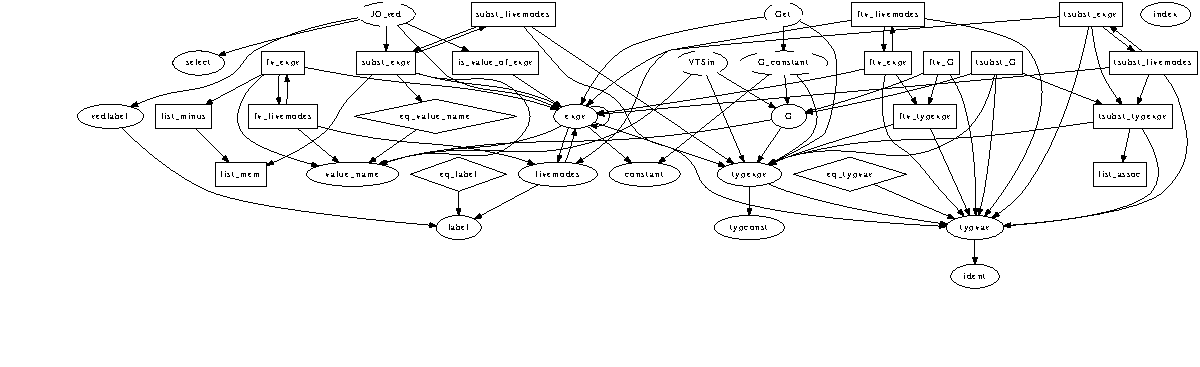
\includegraphics[width=\linewidth]{coqBaseStruct.pdf}
\caption{Dependencies in the Coq semantics}
\label{fig:coqBaseStruct}
\end{figure}
In \Cref{fig:coqBaseStruct} I detail the dependencies between different parts of the Coq version of the semantics. There are four types of objects in the Coq file:
\begin{enumerate}
\item{Inductive sets: they are the inductive data structures. These are the expression grammar objects mentioned in \Cref{fig:grammardep} with the same structure and the types of metavariables. Inductive sets are denoted by ovals with solid outlines. As an example, type expressions are translated from the Ott version in \Cref{lst:otttypexpr} to the Coq equivalent in \Cref{lst:coqtypexpr}. Simple grammars generate a set of tagged variants. 


\begin{lstlisting}[language={Ott}, caption={Ott type expressions}, label={lst:otttypexpr}]
typexpr, t :: TE_ ::=
  | typconst                           ::   :: constants
  | typvar                             ::   :: var
  | typexpr -> typexpr'                ::   :: arrow
  | typexpr '*' typexpr'               ::   :: prod
  | con typexpr                        ::   :: concurrent
  | typexpr '+' typexpr'               ::   :: sum
  | ( typexpr )                        :: S :: paren {{ ich [[typexpr]] }} {{ ocaml [[typexpr]] }}
\end{lstlisting}

\begin{minipage}{\linewidth}
\begin{lstlisting}[language={Coq},caption={Coq type expr}, label={lst:coqtypexpr}]
Inductive typexpr : Set := 
 | TE_constants (typconst5:typconst)
 | TE_var (typvar5:typvar)
 | TE_arrow (typexpr5:typexpr) (typexpr':typexpr)
 | TE_prod (typexpr5:typexpr) (typexpr':typexpr)
 | TE_concurrent (typexpr5:typexpr)
 | TE_sum (typexpr5:typexpr) (typexpr':typexpr).
\end{lstlisting}
\end{minipage}
}
\item{Fixpoints, the functions in Coq: The functions in this are all automatically generated from the Ott file. The most important ones are the expression substitution, free variable, value check fixpoints. The script also includes a few functions supporting the previous ones. Fixpoints are denoted by rectangles. The value subgrammar is translated as a fixpoint over expressions. 

\begin{lstlisting}[language={Ott}, caption={Ott value subgrammar}, label={lst:ottvaluesub}]
value, v :: V_ ::=
  | constant                           ::   :: constant
  | function value_name : typexpr -> expr        ::   :: function
  | live lm                         ::   :: live_expr
  | inl v                              ::   :: taggedleft
  | inr v                              ::   :: taggedright
  | { v , v' }                         ::   :: valuepair
  | ( v )                             :: S :: paren {{ ich [[v]] }} {{ ocaml [[v]] }}
\end{lstlisting}

\begin{minipage}{\linewidth}
\begin{lstlisting}[language={Coq},caption={Coq value subgrammar}, label={lst:coqvaluesub}, escapeinside={@}{@}]
Fixpoint is_value_of_expr (e_5:expr) : Prop :=
  match e_5 with
  | (E_ident value_name5) => False
  | (E_constant constant5) => (True)
(* Manual change *)
@\label{lst:coqhandmod}@  | (E_apply expr5 expr') => match expr5 with | E_constant (CONST_fork) => is_value_of_expr (expr') | E_constant (CONST_pair) => is_value_of_expr (expr') | _ => False end  
  | (E_bind expr5 expr') => False
  | (E_function value_name5 typexpr5 expr5) => (True)
  | (E_fix e) => False
  | (E_live_expr lm) => (True)
  | (E_pair e e') => ((is_value_of_expr e) /\ (is_value_of_expr e'))
  | (E_taggingleft e) => ((is_value_of_expr e))
  | (E_taggingright e) => ((is_value_of_expr e))
  | (E_case e1 x1 e2 x2 e3) => False
end.
\end{lstlisting}
\end{minipage}	
Notice however, that I was not able to define the value property of partial applications of primitives \textbf{fork} and \textbf{pair}, therefore I manually changed the incorrect value subgrammar check. Ott offers single and multiple substitution predicates for its destination languages. These are implemented as fixpoints in Coq. As an example, see the expression substitution in \Cref{lst:coqexprsubst}.
\begin{minipage}{\linewidth}
\begin{lstlisting}[language={Coq},caption={Coq expression substitution}, label={lst:coqexprsubst}]
Fixpoint subst_expr (e_5:expr) (x_5:value_name) (e__6:expr) {struct e__6} : expr :=
  match e__6 with
  | (E_ident value_name5) => (if eq_value_name value_name5 x_5 then e_5 else (E_ident value_name5))
  | (E_constant constant5) => E_constant constant5
  | (E_apply expr5 expr') => E_apply (subst_expr e_5 x_5 expr5) (subst_expr e_5 x_5 expr')
  | (E_bind expr5 expr') => E_bind (subst_expr e_5 x_5 expr5) (subst_expr e_5 x_5 expr')
  | (E_function value_name5 typexpr5 expr5) => E_function value_name5 typexpr5 (if list_mem eq_value_name x_5 (cons value_name5 nil) then expr5 else (subst_expr e_5 x_5 expr5))
  | (E_fix e) => E_fix (subst_expr e_5 x_5 e)
  | (E_live_expr lm) => E_live_expr (subst_livemodes e_5 x_5 lm)
  | (E_pair e e') => E_pair (subst_expr e_5 x_5 e) (subst_expr e_5 x_5 e')
  | (E_taggingleft e) => E_taggingleft (subst_expr e_5 x_5 e)
  | (E_taggingright e) => E_taggingright (subst_expr e_5 x_5 e)
  | (E_case e1 x1 e2 x2 e3) => E_case (subst_expr e_5 x_5 e1) x1 (subst_expr e_5 x_5 e2) x2 (subst_expr e_5 x_5 e3)
end
\end{lstlisting}
\end{minipage}	
}
\item{Logical inductive sets: As mentioned previously a logical inductive set is an inductively defined set of propositions. This is the way the reduction relation and the typing relation is represented. Logical inductive sets are represented in \Cref{fig:coqBaseStruct} by ovals with dashed outline. For example a clause in the reduction relation is translated from the simple inference rule presentation in \Cref{lst:ottcontextapp1} to proposition in the logical inductive set \verb|JO_red| in \Cref{lst:coqlogind}.

\begin{lstlisting}[language={Ott}, caption={Ott reduction relation example}, label={lst:ottcontextapp1}]
e [ s ] --> [ rl ] e''
----------------------------  :: context_app1
e e' [ s ] --> [ rl ] e'' e'
\end{lstlisting}

\begin{minipage}{\linewidth}
\begin{lstlisting}[language={Coq},caption={Coq reduction relation example}, label={lst:coqlogind}]
Inductive JO_red : expr -> select -> redlabel -> expr -> Prop :=    (* defn red *)
 | JO_red_context_app1 : forall (e e':expr) (s:select) (rl:redlabel) (e'':expr),
     JO_red e s rl e'' ->
     JO_red (E_apply e e') s rl (E_apply e'' e')
  ...
\end{lstlisting}
\end{minipage}	
}
\item{Lemmas: There are a few supporting lemmas about the equality of variables. These are automatically generated by Ott. Lemmas are denoted with diamonds. An easy example would be the straightforward lemma that says labels are either equal or not in \Cref{lst:coqeqlabel}.

\begin{minipage}{\linewidth}
\begin{lstlisting}[language={Coq},caption={Coq label equality lemma}, label={lst:coqeqlabel}]
Lemma eq_label: forall (x y : label), {x = y} + {x <> y}.
Proof.
  decide equality; auto with ott_coq_equality arith.
Defined.
\end{lstlisting}
\end{minipage}	

}
\end{enumerate} 
The automatically generated Coq representation had a slight issue in that I could not easily define partial application of curried primitive functions as values. Instead, I hand modified the fixpoint in the translated Coq the particular case on \Cref{lst:coqhandmod} in \Cref{lst:coqvaluesub}.
\subsection{Extractable reduction relation}
Coq provides extraction facilities to OCaml and Haskell. However, the built in extraction only deals with inductive sets and fixpoints that do not involve propositions, more specifically the \textit{Prop} sort. There are good reasons why logical inductive definitions are not extracted from Coq. Logical inductive types do not need to conform to any input/output relationship and computations that correspond to a logical inductive relation need not always terminate. Extraction from Coq is required to produce a certification of equivalence and the Calculus of Inductive Constructions, the logic underlying Coq, cannot directly express a certification for a non-terminating program. 


Logical inductive types are often used for description of various concepts in semantics, especially reduction relations. Ott generates a logical inductive relation as seen in \Cref{lst:coqlogind}. For simple relations, like the value relation in \Cref{lst:coqvaluesub} it is simple to rewrite in a set inductive manner. However, for complex non-terminating relations, like the reduction relation in this project, rewriting is not feasible.  Delahaye et al.\cite{delahaye2007extracting,tollitte2012producing} proposed a method of extracting such relations to OCaml by annotating the input/output modes of the elements of the relation. 

I rewrote the value check logical fixpoint to an extractable version by simply replacing the True and False propositions by their boolean counterpart and successfully extracted it by the built-in Coq extraction. However, not even the Coq plugin based on element modes could extract the reduction relation generated by Ott. 

The first issue with the extraction to a functional program was the way the selection argument was supplied. Originally, the required a single selection value. In the case of fork reduction rules this would not be enough to generate a certified program.
\begin{equation}
                                         \inferrule
                                           {e \overset{rl}{\underset{s}{\longrightarrow}} e'}
                                           { \textbf{fork } (\textit{Live expr } e) (\textit{Live } lm)  \overset{rl}{\underset{1}{\longrightarrow}}\\\\ \textbf{fork } (\textit{Live expr } e') (\textit{Live } lm)  } \tag{R-Forkmove1} \label{eq:forkmove1}
                                         \end{equation}
                                            \begin{equation}
                                          \inferrule
                                            {e \overset{rl}{\underset{s}{\longrightarrow}} e'}
                                            { \textbf{fork } (\textit{Live } lm) (\textit{Live expr } e) \overset{rl}{\underset{2}{\longrightarrow}}\\\\ \textbf{fork }  (\textit{Live } lm) (\textit{Live expr } e')  } \tag{R-Forkmove2} \label{eq:forkmove2}
                                           \end{equation}
The extracted program would have to somehow pick a possible value for $ s $ in $ e \overset{rl}{\underset{s}{\longrightarrow}} e' $ while it is only supplied with the value 1. Clearly always picking one or the other would not be satisfactory. As I had no way of choosing it non-deterministically, I wanted the argument to fully describe all $ s $ values the system used. I opted for a co-inductive stream of selections because there can be an arbitrary number of \textbf{fork}s nested in each other with arbitrary number of selection values to make a single step . 

\begin{minipage}{\linewidth}
\begin{lstlisting}[language={Coq},caption={Coq co-inductive selection sequence}, label={lst:coqselectstar}]
CoInductive selectstar : Set := Seq : select -> selectstar -> selectstar.
\end{lstlisting}
\end{minipage}

Co-inductive data structures represent potentially infinite data and featured in a number of programming languages: lazy lists, trees and streams all describe co-inductive structures. In \Cref{lst:coqselectstar} I define \verb|selectstar| where each element is pair of a selection value and a further \verb|selectstar| representing the rest of the selection values.  With an infinite sequence of selection values the program can make arbitrary many decisions and it is extractable.

The second problem that surfaced was that the extraction plugin does not generate code that backtracks from a case where we invoked the reduction relation on an internal part. If an expression $ e $ does not reduce and the extracted reduction function is invoked it will fail with an \lstinline|assert false|. I chose to add a logically superfluous assumption of expression $ e $ not being a value. This assumption is superfluous as an expression that reduces cannot be a value by the \verb|red_not_value| theorem.  \Cref{lst:coqredunsafe,lst:coqxredsafe} are a good example of how this transformation happens. \vspace{4mm}

\begin{minipage}{0.9\linewidth}
\begin{lstlisting}[language={Coq},caption={Coq reduction clause with unsafe assumption}, label={lst:coqredunsafe}]
| JO_red_evalbind : forall (e e'':expr) (s:select) (rl:redlabel) (e':expr),
     JO_red e s rl e' ->
     JO_red (E_bind e e'') s rl (E_bind e' e'')
\end{lstlisting}
\end{minipage}

\begin{minipage}{\linewidth}
\begin{lstlisting}[language={Coq},caption={Coq extractable reduction clause with safe assumption}, label={lst:coqxredsafe}]
 | XJO_red_evalbind : forall (e e'' e':expr) (s:selectstar),
    (eq (xis_value_of_expr e) false) ->
     XJO_red e s e' ->
     XJO_red (E_bind e e'') s (E_bind e' e'')
\end{lstlisting}
\end{minipage}


The last issue was due to the experimental nature of the plugin: the optimisations and inference algorithm ran out of stack space when invoked with all 26 rules. Therefore I extracted in three parts and recombined them by hand.

\section{OCaml system}
In this section I give a brief outline of the structure of the extracted OCaml, how it is modified to be runnable and a brief overview of potential syntactic sugar that can be used to aid development in the framework. 
\begin{figure}
\centering
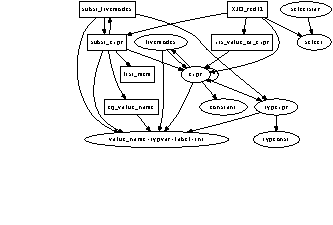
\includegraphics[width=\linewidth]{ocamlBaseStruct.pdf}
\caption{Dependencies in the OCaml code}
\label{fig:ocamlBaseStruct}
\end{figure}
\subsection{Outline of the OCaml code}
The OCaml code consists of the extracted versions of the following:
\begin{itemize}
\item{Inductive sets like expressions, constants and type expressions as tagged variants. These are represented as ovals in \Cref{fig:ocamlBaseStruct}.}
\item{Functions like the expression substitution or XJO\_red12, the reduction function. These are the rectangles in \Cref{fig:ocamlBaseStruct}.}
\item{The metavariables \verb|value_name, label, ident| are all of OCaml type \lstinline|int| instead of constructor based extractions of Coq \lstinline[language={Coq}]|nat|. This has the caveat that \lstinline|int| may overflow or represent negative numbers, while the Coq \lstinline[language={Coq}]|nat| cannot. Realistically, no program would have this problem.}
\end{itemize}
Their interdependence is shown on \Cref{fig:ocamlBaseStruct}. 
\subsection{Hand modifications and justifications}
I have made a number of modifications to the OCaml code to make it runnable. This includes changing the type of labels from int to $ \textbf{unit}\rightarrow\textbf{unit} $ and inserting terms in the relevant cases to run these computations. 

Furthermore I have changed the way \verb|selectstar| is implemented. The extraction results in the type in \Cref{lst:ocamllazystar} which involves the Lazy module of OCaml. While the extraction of co-inductive types to lazy types is sound, for simplicity I used a simple lazy stream in \Cref{lst:ocamlstreamstar}. 

\begin{minipage}{\linewidth}
\begin{lstlisting}[caption={OCaml lazy selectstar}, label={lst:ocamllazystar}]
type selectstar = __selectstar Lazy.t
and __selectstar =
| Seq of select * selectstar
\end{lstlisting}
\end{minipage}

\begin{minipage}{\linewidth}
\begin{lstlisting}[caption={OCaml stream selectstar}, label={lst:ocamlstreamstar}]
type selectstar = | Seq of select * (unit -> selectstar) 
\end{lstlisting}
\end{minipage}

As the extraction plugin is experimental there were a number of inefficiencies and a few issues due to the fact that the semantics of OCaml pattern matching is sequential, while it is parallel in Coq. While Tollitte\cite{tollitte2012producing} made progress on the merging of cases when one case subsumes the other, these were not always correctly identified. For example the case \Crefrange{lst:ocamlvalexpappcaseStart}{lst:ocamlvalexpappcaseEnd} in \Cref{lst:ocamlorigapp} subsumes the case \Cref{lst:ocamlorigsub}. The plugin was unable to infer this as that would have required it to show that function term is always a value, regardless of its parameters. This is an issue as any function with a parameter that can be reduced will fail, as the case in \Cref{lst:ocamlorigsub} comes first.

\begin{minipage}{\linewidth}
\begin{lstlisting}[caption={OCaml original substitution case}, label={lst:ocamlorigsub}]
  | (E_apply (E_function (x, t, e), v), s) ->
    (match xis_value_of_expr v with
     | true -> subst_expr v x e
     | _ -> assert false (*  *))
\end{lstlisting}
\end{minipage}

\begin{minipage}{\linewidth}
\begin{lstlisting}[caption={OCaml original application case}, label={lst:ocamlorigapp}, escapeinside={@}{@}]
  | (E_apply (e, e'), s) ->
    (match xis_value_of_expr e with
     | false ->
 @\label{lst:ocamlunneededmatchonfun}@      (match xJO_red12 e s with
        | e'' -> E_apply (e'', e')
        | _ -> assert false (*  *))
 @\label{lst:ocamlvalexpappcaseStart}@    | true ->
       (match xJO_red12 e' s with
        | e'' -> E_apply (e, e'')
 @\label{lst:ocamlvalexpappcaseEnd}@       | _ -> assert false (*  *))
 @\label{lst:ocamlunneededdefault2}@    | _ -> assert false (*  *))
\end{lstlisting}
\end{minipage}
My solution was to insert the correct step into the failing match as in \Cref{lst:ocamlfixsub}. Note, that taking that reduction may fail, but that is the expected behaviour.
\begin{minipage}{\linewidth}
\begin{lstlisting}[caption={OCaml fixed substitution case}, label={lst:ocamlfixsub}]
  | (E_apply (E_function (x, t, e), v), s) ->
    (match xis_value_of_expr v with
     | true -> subst_expr v x e
     | false -> E_apply (E_function (x, t, e), (xJO_red12 v s)))
\end{lstlisting}
\end{minipage}
A reoccurring inefficiency comes from the extraction plugin generating a default failing case in all situations, even if the default case may never happen. \Cref{lst:ocamlunneededdefault2} in \Cref{lst:ocamlorigapp} is an example of this: a boolean may only take the values true or false. A similar issue occurs when evaluating a function:  \Cref{lst:ocamlunneededmatchonfun} in the same listing matches by giving a name to the return value, but generates a default case as well. To this latter problem I simply removed the match and replaced the name of the return value with the function call.

A further issue occurs when occasionally the plugin reorders matches on assumptions. Even though the safe assumption was inserted in the case in \Cref{lst:ocamlswapassume} it was reordered by the plugin to come after the unsafe assumption. 
\begin{minipage}{\linewidth}
\begin{lstlisting}[caption={OCaml swapped assumptions}, label={lst:ocamlswapassume}]
  | (E_bind (e, e''), s) ->
    (match xJO_red12 e s with
     | e' ->
       (match xis_value_of_expr e with
        | false -> E_bind (e', e'')
        | _ -> assert false (*  *))
     | _ -> assert false (*  *))
\end{lstlisting}
\end{minipage}
The simple solution to this is to swap the assumptions, however in some cases that leads to to the issues mentioned above.
\subsection{Syntactic sugar}
Due to the multiple layers of automatic naming developing in this framework directly could be cumbersome. I have defined a few OCaml functions to serve as syntactic sugar. The two broad categories of sugar are syntax to build expressions and schedulers. 
\begin{itemize}
\item{Boxing expressions and computations: \lstinline|let boxe e = E_live_expr (LM_expr e)|, \lstinline|let boxc f = E_live_expr (LM_comp f)|}
\item{An infix bind operator: \lstinline|let ( >>= ) a b = E_bind (a, b)|}
\item{Application: \lstinline|let app a b = E_apply (a, b)|}
\item{Fork: \lstinline|let fork a b = app ( app (E_constant CONST_fork) a ) b|}
\item{Round-robin and random schedulers in \Cref{lst:ocamlrrsched} and \Cref{lst:ocamlrandsched} respectively.}
\end{itemize}
\begin{minipage}{\linewidth}
\begin{lstlisting}[caption={OCaml round-robin scheduler}, label={lst:ocamlrrsched}]
  let rec makerr1 () = Seq(S_First, makerr2) 
  and makerr2 () = Seq(S_Second, makerr1) 
  
  let rec evalrr1 e n = (match n with 
           | 0 -> e
           | m -> evalrr2 (xJO_red12 e (makerr1 ())) (m-1))
  and evalrr2 e n = (match n with 
           | 0 -> e
           | m -> evalrr1 (xJO_red12 e (makerr2 ())) (m-1))
\end{lstlisting}
\end{minipage}
\begin{minipage}{\linewidth}
\begin{lstlisting}[caption={OCaml random scheduler}, label={lst:ocamlrandsched}]
  let rec makerand () = if Random.bool() then Seq(S_First, makerand) else Seq(S_Second, makerand)
  
  let rec evalrand e n = (match n with 
                       | 0 -> e
                       | m -> evalrand (xJO_red12 e (makerand ())) (m-1))
\end{lstlisting}
\end{minipage}


\cleardoublepage
\chapter{Evaluation}

\section{Theoretical evaluation}
Properties to evaluate: monadic laws, fork commutativity and associativity (liveness ?), type preservation and progress ?.

\subsection{Methods}
\subsubsection{Weak bisimilarity}
Intro to weak bisimilarity.


What form does a general weak bisimilarity proof take.


How does it appear here.
\subsection{Properties}
\subsubsection{Monadic laws}

\[ \textbf{ret } v\,\gg=\, e\quad \simeq \quad e\,v \]
\[  \textit{Live expr }v\,\gg=\, \textbf{ret}\quad \simeq \quad \textit{Live expr }v \]

\[ (\textit{Live expr }v\, \gg=\, f) \, \gg=\, g \quad \simeq \quad \textit{Live expr }v\, \gg=\, (\lambda x. (f\, v) \, \gg=\, g ) \]

\subsubsection{Fork commutativity}
Outline of fork commutativity
\[ a\,|\,b\quad\simeq\quad b \, | \, a \]
\subsubsection{Fork associativity}
Fork in this implementation is not associative:
\subsubsection{Deadlock properties}
\[ \delta \, |\, x \quad \simeq \quad x \]
\[ \delta \, \gg=\, e\quad \simeq \quad \delta \]
\subsubsection{Remarks on congruence}
\subsubsection{Type preservation?}
\subsubsection{Progress?} 
%Theoretical evaluation
% - Monadic laws
% - Fork commutativity
% - Fork associativity (limited?)
% - Liveness ?
% - Type preservation ?
% - Progress

% Practical evaluation
\section{Practical evaluation}
Evaluation of speed and memory requirements absolutely and relative to implementations in LWT and Async.
\subsection{Methods}
\subsection{Examples}
\subsubsection{Kahn process network}
\subsubsection{Eratosthene Sieve}
\subsubsection{Concurrent sort}
%

\cleardoublepage
\chapter{Conclusion}

I hope that this rough guide to writing a dissertation is \LaTeX\ has
been helpful and saved you time.




\cleardoublepage

%%%%%%%%%%%%%%%%%%%%%%%%%%%%%%%%%%%%%%%%%%%%%%%%%%%%%%%%%%%%%%%%%%%%%
% the bibliography

\addcontentsline{toc}{chapter}{Bibliography}
\bibliography{refs}
\cleardoublepage

%%%%%%%%%%%%%%%%%%%%%%%%%%%%%%%%%%%%%%%%%%%%%%%%%%%%%%%%%%%%%%%%%%%%%
% the appendices
\appendix

\chapter{Full semantics}
\label{chap:fullsemantics}
\includepdf[pages=-]{../mconbase.pdf}

\section{blah}
%\section{proposal.tex}
%{\scriptsize\verbatiminput{proposal.tex}}

%\section{propbody.tex}
%{\scriptsize\verbatiminput{propbody.tex}}



%\cleardoublepage

%\chapter{Makefile}

%\section{\label{makefile}Makefile}
%{\scriptsize\verbatiminput{makefile.txt}}

%\section{refs.bib}
%{\scriptsize\verbatiminput{refs.bib}}


\cleardoublepage

\chapter{Project Proposal}



\section{Introduction of work to be undertaken}
With the rise of ubiquitous multiple core systems it is necessary for a working programmer to use concurrency to the greatest extent. However concurrent code has never been easy to write as human reasoning is often poorly equipped with the tools necessary to think about such systems. That is why it is essential for a programming language to provide safe and sound primitives to tackle this problem. 

My project aims to do this in the OCaml\cite{OCaml} language by developing a lightweight cooperating threading framework that holds correctness as a core value. The functional nature allows the use of one of the most recent trends in languages popular in academia, monads, to be used for a correct implementation. 

There have been two very successful frameworks, LWT\cite{LWT} and Async\cite{Async} that both provided the primitives for concurrent development in OCaml however neither is supported by a clear semantic description as their main focus was ease of use and speed. 
\section{Description of starting point}
My personal starting points are the courses ML under Windows (IA), Semantics of Programming Languages (IB), Logic and Proof (IB) and Concepts in Programming Languages (IB). Furthermore I have done extracurricular reading into semantics and typing and attended the Denotational Semantics (II) course in the past year.

The preparatory research period has to include familiarising myself with OCaml and the chosen specification and proof assistant tools.
\section{Substance and structure}
The project will consist of first creating a formal specification for a simple monad that has three main operations bind, return and choose. The behaviour of these operations will be specified in a current semantics tool like Lem\cite{Lem} or Ott\cite{Ott}. 

As large amount of research has gone into both monadic concurrency and implementations in OCaml, the project will draw inspiration from Claessen\cite{Claessen99functionalpearls}, Deleuze\cite{deleuzelight} and Vouillon\cite{vouillon2008lwt}.

Some atomic, blocking operations will also be specified including reading and writing to a console prompt or file to better illustrate the concurrency properties and make testing and evaluation possible.

This theory driven executable specification will be paired by a hand implementation and will be thoroughly checked against each other to ensure that both adhere to the desired semantics. 

Both of these implementations will be then compared against the two current frameworks for simplicity and speed on various test cases.

If time allows, an extension will also be carried out on the theorem prover version of the specification to formally verify that the implementation is correct. 
\section{Criteria}
For the project to be deemed a success the following items must be
successfully completed.
\begin{enumerate}
\item A specification for a monadic concurrency framework must be designed in the format of a semantics tool.
\item This specification needs to be exported to a proof assistant and has a runnable OCaml version
\item Test cases must be written that can thoroughly check a concurrency framework
\item A hand implementation needs to be designed, implemented and tested against the specification
\item The implementations must be compared to the frameworks LWT and Async based on speed
\item The dissertation must be planned and written
\end{enumerate}

In case the extension will also become viable then its success criterion is that there is a clear formal verification accompanying the automated theorem prover version of the specification.
\section{Timetable}
The project will be split into two week packages


\subsection{Week 1 and 2}
Preparatory reading and research into tools that can be used for writing the specification and in the extension, the proofs. The tools of choice at the time of proposal are Ott for the specification step and Coq\cite{Coq} as the proof assistant. Potentially a meeting arranged in the Computer Lab by an expert in using these tools. 

\textbf{Deliverable:} Small example specifications to try out the tool chain, including SKI combinator calculus.

\subsection{Week 3 and 4}
Investigating the two current libraries and their design decisions and planning the necessary parts of specification. Identifying the test cases that are thorough and common in concurrent code.

\textbf{Deliverable:} A document describing the major design decisions of the two libraries, the difference in design of the specification and a set of test cases much like the ones used in OCaml Light \cite{OCamlLight, OCamlLightWeb}, but with a concurrency focus.

\subsection{Week 5 and 6}
Writing the specification and exporting to automated theorem provers and OCaml.

\textbf{Deliverable:} The specification document in the format of the semantics tool and exported in the formats of the proof assistant and OCaml.


\subsection{Week 7 and 8}
Hand implement a version that adheres to the specification and test it against the runnable semantics.

\subsection{Week 9 and 10}
Evaluating the implementations of the concurrency framework against LWT and Async.
Writing up the halfway report.

\textbf{Deliverable:} Evaluation data and charts, the halfway report.
\subsection{Week 11 and 12}
If unexpected complexity occurs these two weeks can be used to compensate, otherwise starting on the verification proof in the proof assistant.
\subsection{Week 13 and 14}
If necessary adding more primitives (I/O, network) to test with, improving performance and finishing the verification proof. If time allows writing guide for future use of the framework.
\subsection{Week 15 and 16}
Combining all previously delivered documents as a starting point for the dissertation and doing any necessary further evaluation and extension.
Creating the first, rough draft of the dissertation.
\subsection{Week 17 and 18}
Getting to the final structure but not necessarily final wording of the dissertation, acquiring all necessary graphs and charts, incorporating ongoing feedback from the supervisor.
\subsection{Week 19 and 20}
Finalising the dissertation and incorporating all feedback and polishing. 
\section{Resource Declaration}
The project will need the following resources:
\begin{itemize}
\item MCS computer access that is provided for all projects
\item The OCaml core libraries and compiler
\item The LWT and Async libraries
\item The Lem tool
\item The Ott tool
\item The use of my personal laptop, to work more efficiently
\end{itemize}

As my personal laptop is included a suitable back-up plan is necessary which will consist of the following:
\begin{itemize}
\item A backup to my personal Dropbox account
\item A Git repository on Github
\item Frequent backups (potentially remotely) to the MCS partition
\end{itemize}
My supervisor and on request my overseers will receive access to both the Dropbox account and Github repository to allow full transparency.


\begin{thebibliography}{9}

\bibitem{OCaml}
 OCaml.
 \emph{http://ocaml.org/}

\bibitem{LWT}
 LWT, Lightweight Threading library.
 \emph{http://ocsigen.org/lwt/}

\bibitem{Async}
 Async, Open source concurrency library by Jane Street
 \emph{http://janestreet.github.io/}
 
 \bibitem{Lem}
 Lem, a tool for lightweight executable mathematics.\newline
 \emph{http://www.cs.kent.ac.uk/people/staff/sao/lem/}
 
 \bibitem{Ott}
  Ott, a tool for writing definitions of programming languages and calculi.
  Francesco Zappa Nardelli, Peter Sewell, and Scott Owens.\newline
 \emph{http://www.cl.cam.ac.uk/\textasciitilde pes20/ott/}

\bibitem{Claessen99functionalpearls}
  Claessen, Koen.
  \emph{Functional Pearls: A Poor Man's Concurrency Monad}.
  1999.

\bibitem{deleuzelight}
  Deleuze, Christophe.
  \emph{Light Weight Concurrency in OCaml: Continuations, Monads, Promises, Events}.

\bibitem{vouillon2008lwt}
  Vouillon, J{\'e}r{\^o}me.
  \emph{Lwt: a cooperative thread library} in Proceedings of the 2008 ACM SIGPLAN workshop on ML, pages 3--12.
  2008.
  ACM.
 
\bibitem{Coq}
 Coq proof assistant.
 \emph{http://coq.inria.fr/}

\bibitem{OCamlLight}  
 Owens, Scott.
 \emph{A sound semantics for OCaml light.} in Programming Languages and Systems, pages 1--15.
 2008.
 Springer Berlin Heidelberg.
 
\bibitem{OCamlLightWeb}
 Owens, Scott,
 \emph{http://www.cl.cam.ac.uk/\textasciitilde so294/ocaml/}.
 2008.
 


\end{thebibliography}


\end{document}
